\documentclass[journal]{IEEEtran}
\usepackage[a5paper, margin=10mm]{geometry}
%\usepackage{lmodern} % Ensure lmodern is loaded for pdflatex
\usepackage{tfrupee} % Include tfrupee package

\setlength{\headheight}{1cm}
\setlength{\headsep}{0mm}

\usepackage{gvv-book}
\usepackage{gvv}
\usetikzlibrary{patterns}
\lstset{aboveskip=12pt}
\usepackage[center]{caption}
\raggedbottom

\hypersetup{
    colorlinks=true,
    urlcolor=black
}
\usepackage{amsfonts}
\makeindex

\begin{document}
\bibliographystyle{IEEEtran}
\onecolumn

\title{
    \begin{center}
        Math for EE
        \\
        \rule{0.4\columnwidth}{0.4pt}
    \end{center}
}
\author{
    \vspace{11cm}
    \begin{center}
        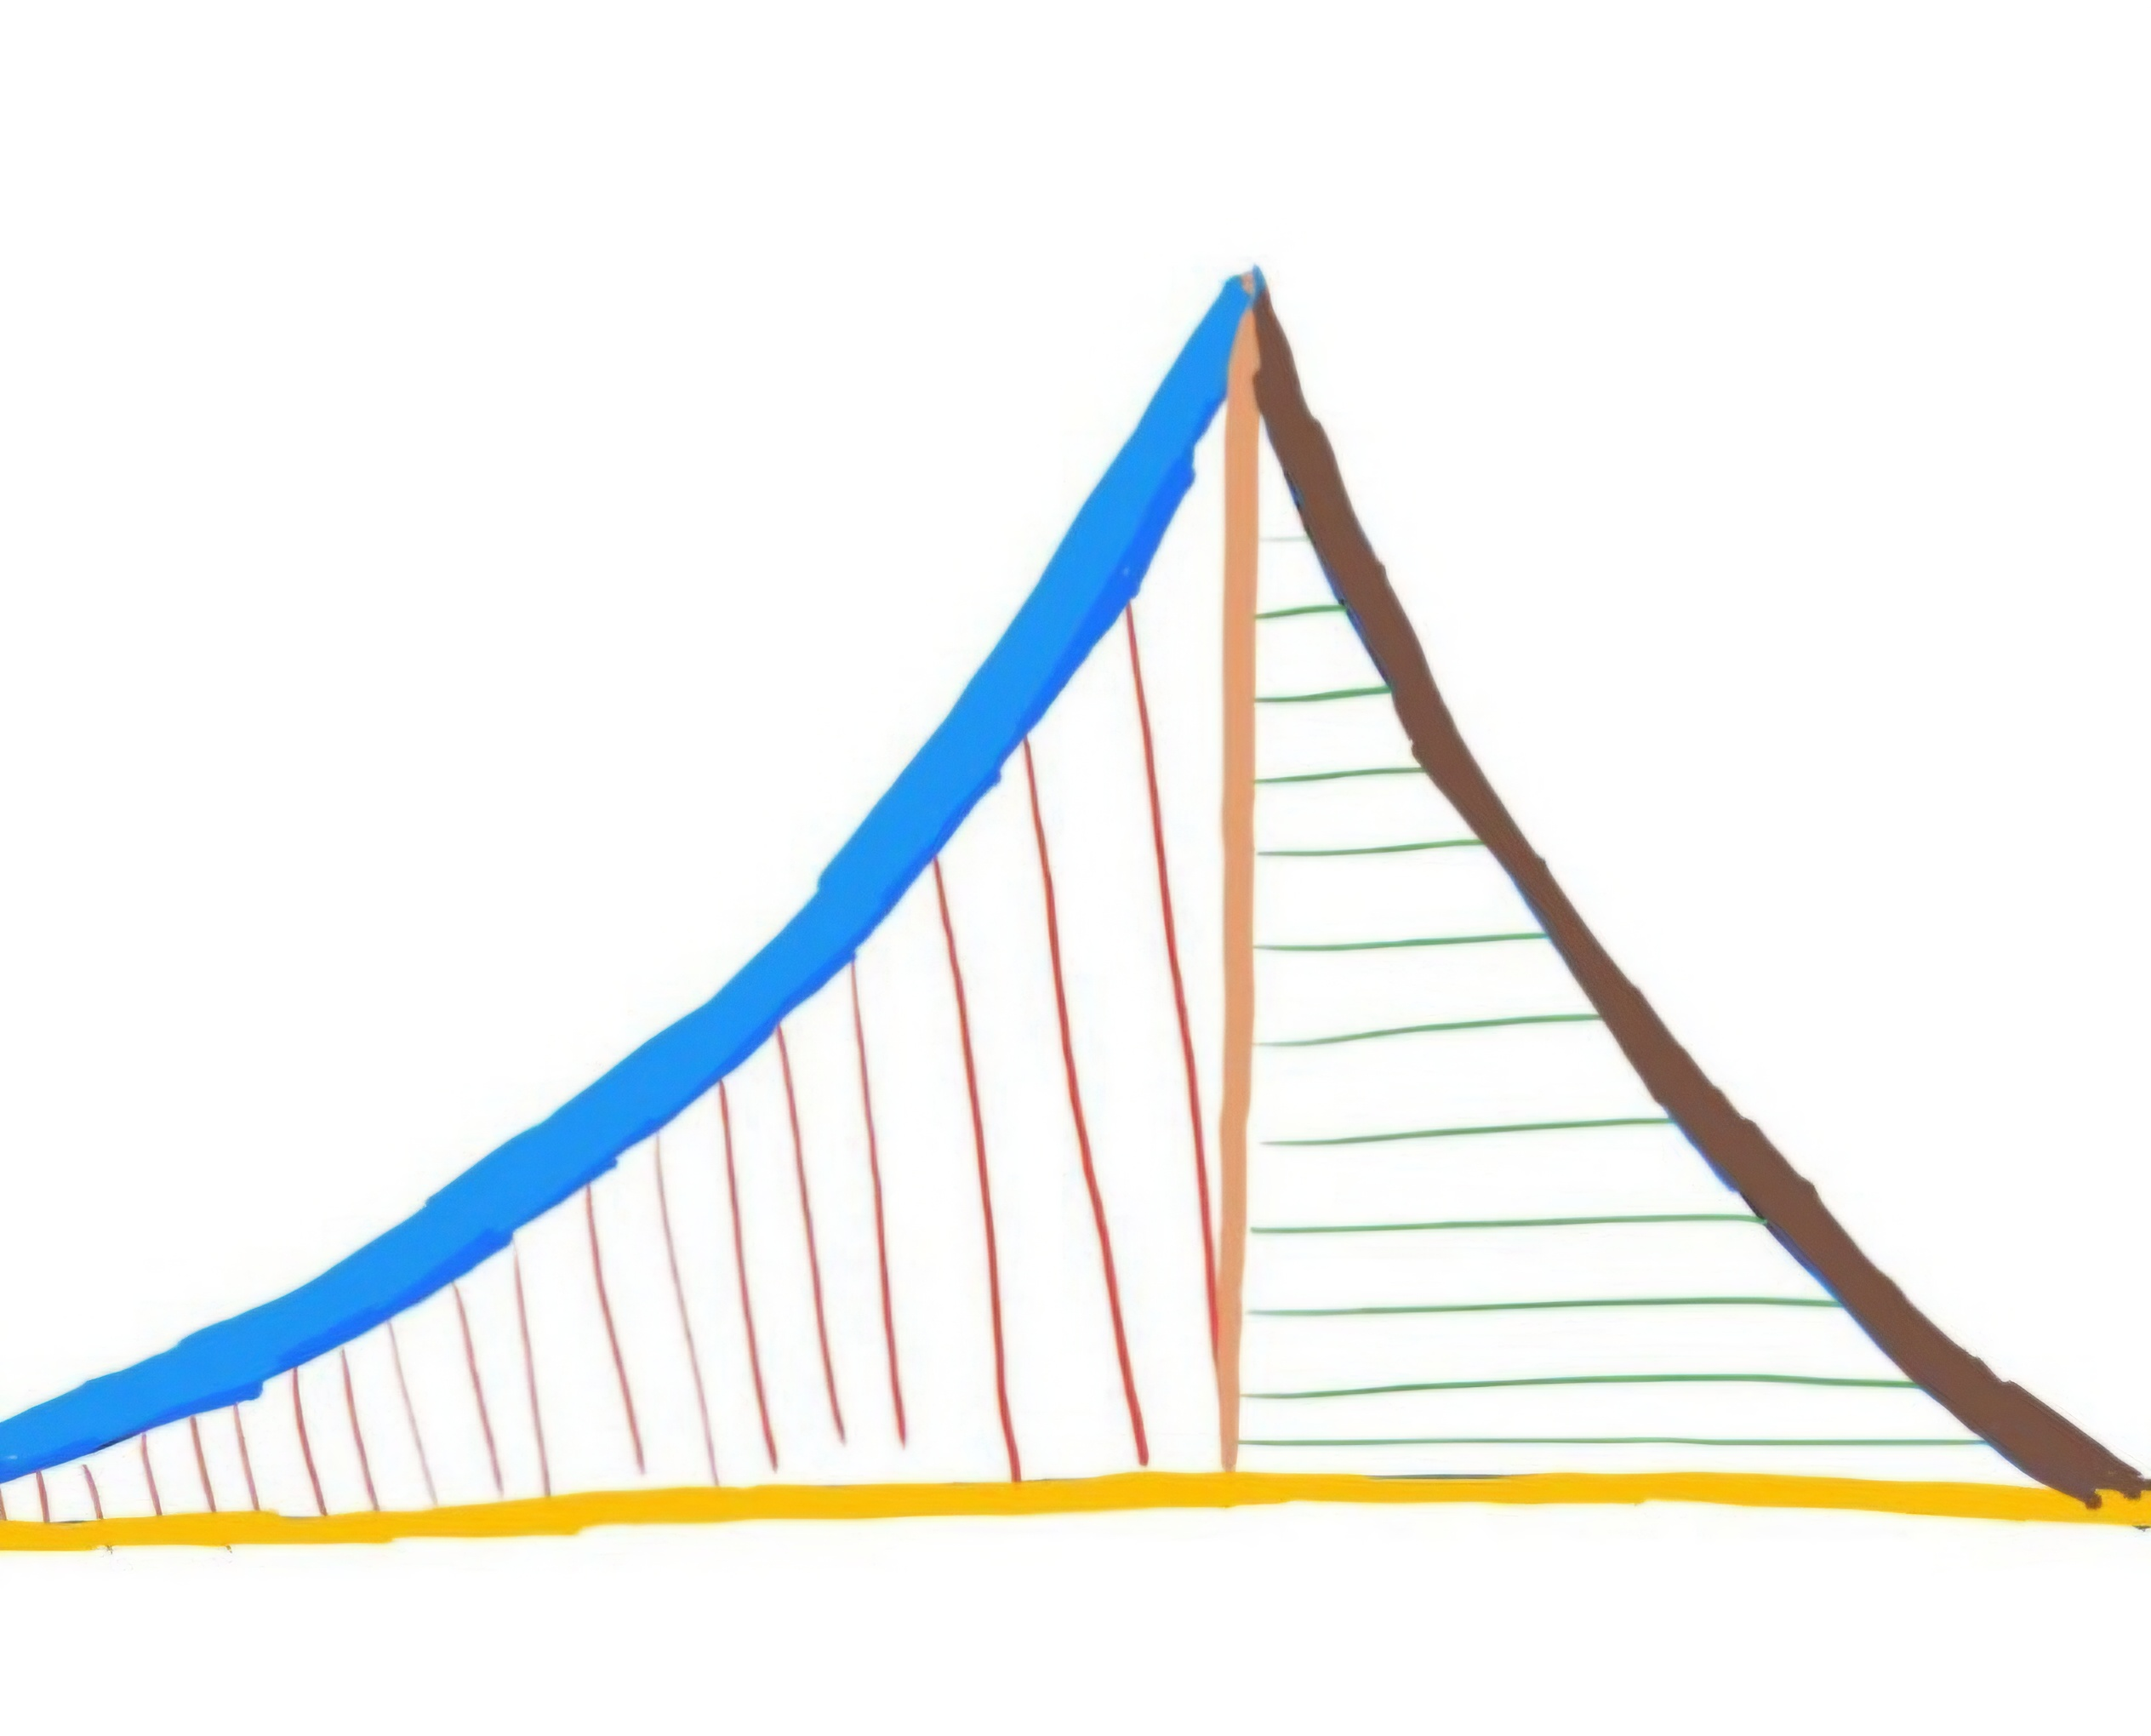
\includegraphics[width=0.2\columnwidth]{figs/logo.jpg}
        \\
        {\huge G. V. V. Sharma}
    \end{center}
}
\maketitle

\newpage
\section*{About this Book}

This book introduces matrices through high school coordinate geometry.
This approach makes it easier for beginners to learn Python for scientific
computing. All problems in the book are from NCERT mathematics textbooks
from Class 9--12. Exercises are from CBSE board exam papers.

The content is sufficient for industry jobs and covers nearly all matrix
prerequisites for machine learning. There is no copyright, so readers are
free to print and share.
License: https://creativecommons.org/licenses/by-sa/3.0/
\\
and
\\
https://www.gnu.org/licenses/fdl-1.3.en.html
\\
First manual appeared in January 2018
\\
First edition published on July 10, 2024
\\
In this edition, some incorrect solutions were removed. All figures
redrawn. More problems added.

\newpage
\onecolumn
\begin{center}
{\Large\bfseries CBSE 2026 10th class maths solutions (65-3-1)}
\end{center}
\vspace{0.4em}

\begin{list}{}{\setlength{\leftmargin}{1.15cm}\setlength{\labelwidth}{1.0cm}\setlength{\labelsep}{0.15cm}\setlength{\itemindent}{0pt}\setlength{\listparindent}{0pt}\setlength{\parsep}{0pt}\setlength{\topsep}{0pt}}
\item[3.1.1] The roots of the quadratic equation $(x-1)^2=16$ are:

\noindent (A) $5,3$ \hfill (B) $4,-4$ \hfill (C) $5,-3$ \hfill (D) $-5,3$

\vspace{0.6em}\par\noindent\textbf{Solution:}

Taking square roots gives $x-1=\pm4$, so $x=5$ or $x=-3$. The correct answer is \textbf{(C)}. The code plots the parabola and the line whose intersections give the roots.
\begin{lstlisting}[frame=single, basicstyle=\rmfamily, escapeinside={(*@}{@*)}]
(*@\makebox[\dimexpr\linewidth-2\fboxsep-2\fboxrule\relax][c]{codes/3.1.1.py}@*)
\end{lstlisting}
\begin{figure}[H]
    \centering
    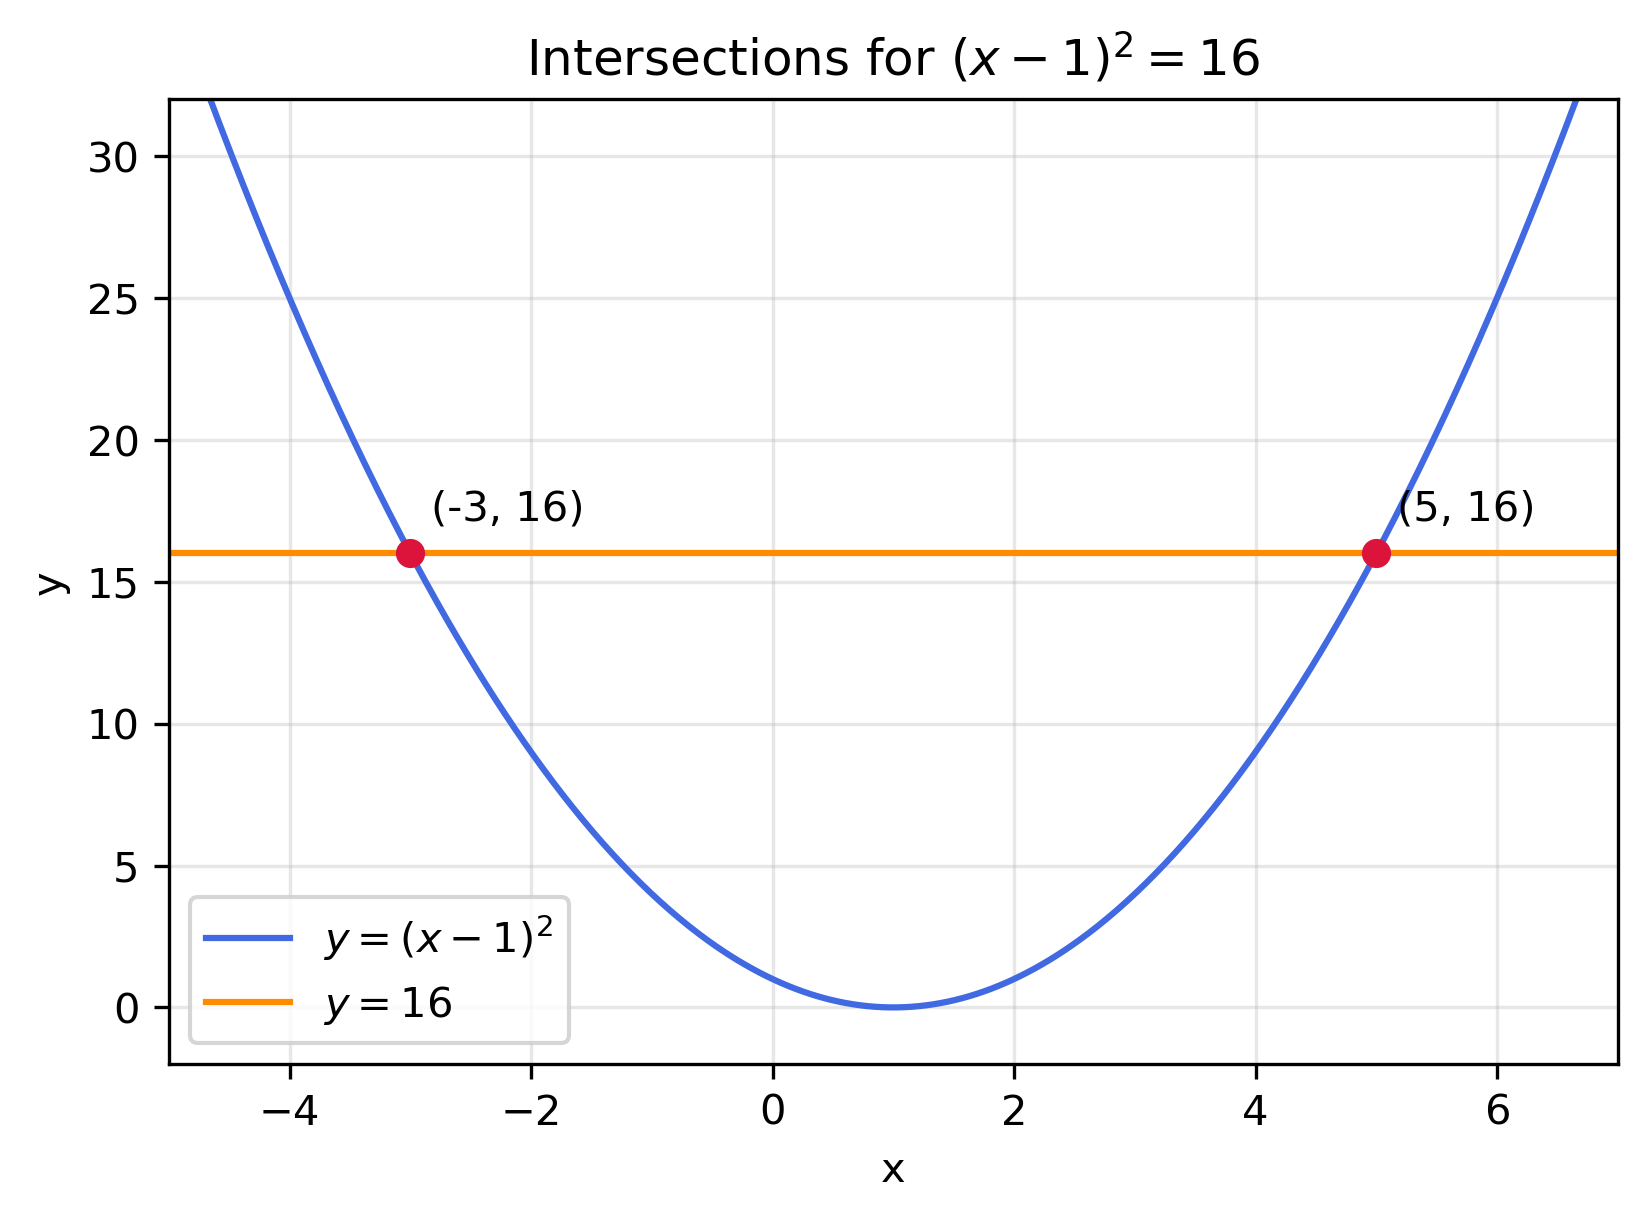
\includegraphics[width=0.48\linewidth]{figs/3.1.1.png}
    \caption{The intersections of $y=(x-1)^2$ and $y=16$.}
\end{figure}

\item[3.1.2] In the figure, $PQ$ and $PR$ are tangents to a circle with centre $O$ and radius $3$ cm. If $\angle QPR=60^\circ$, find the length of each tangent.

\noindent (A) $3\sqrt3$ cm \hfill (B) $3$ cm \hfill (C) $6$ cm \hfill (D) $\sqrt3$ cm

\vspace{0.6em}\par\noindent\textbf{Solution:}

The line $OP$ bisects the angle between the equal tangents, so $\angle QPO=30^\circ$. Since $OQ\perp PQ$ and $OQ=3$ cm,
\[
\tan30^\circ=\frac{OQ}{PQ}\quad\Longrightarrow\quad PQ=3\sqrt3\text{ cm}.
\]
Tangents from $P$ are equal, hence $PR=PQ=3\sqrt3$ cm. The correct answer is \textbf{(A)}.

The code draws the circle, both tangent segments and radii, and calculates their lengths.
\begin{lstlisting}[frame=single, basicstyle=\rmfamily, escapeinside={(*@}{@*)}]
(*@\makebox[\dimexpr\linewidth-2\fboxsep-2\fboxrule\relax][c]{codes/3.1.2.py}@*)
\end{lstlisting}
\begin{figure}[H]
    \centering
    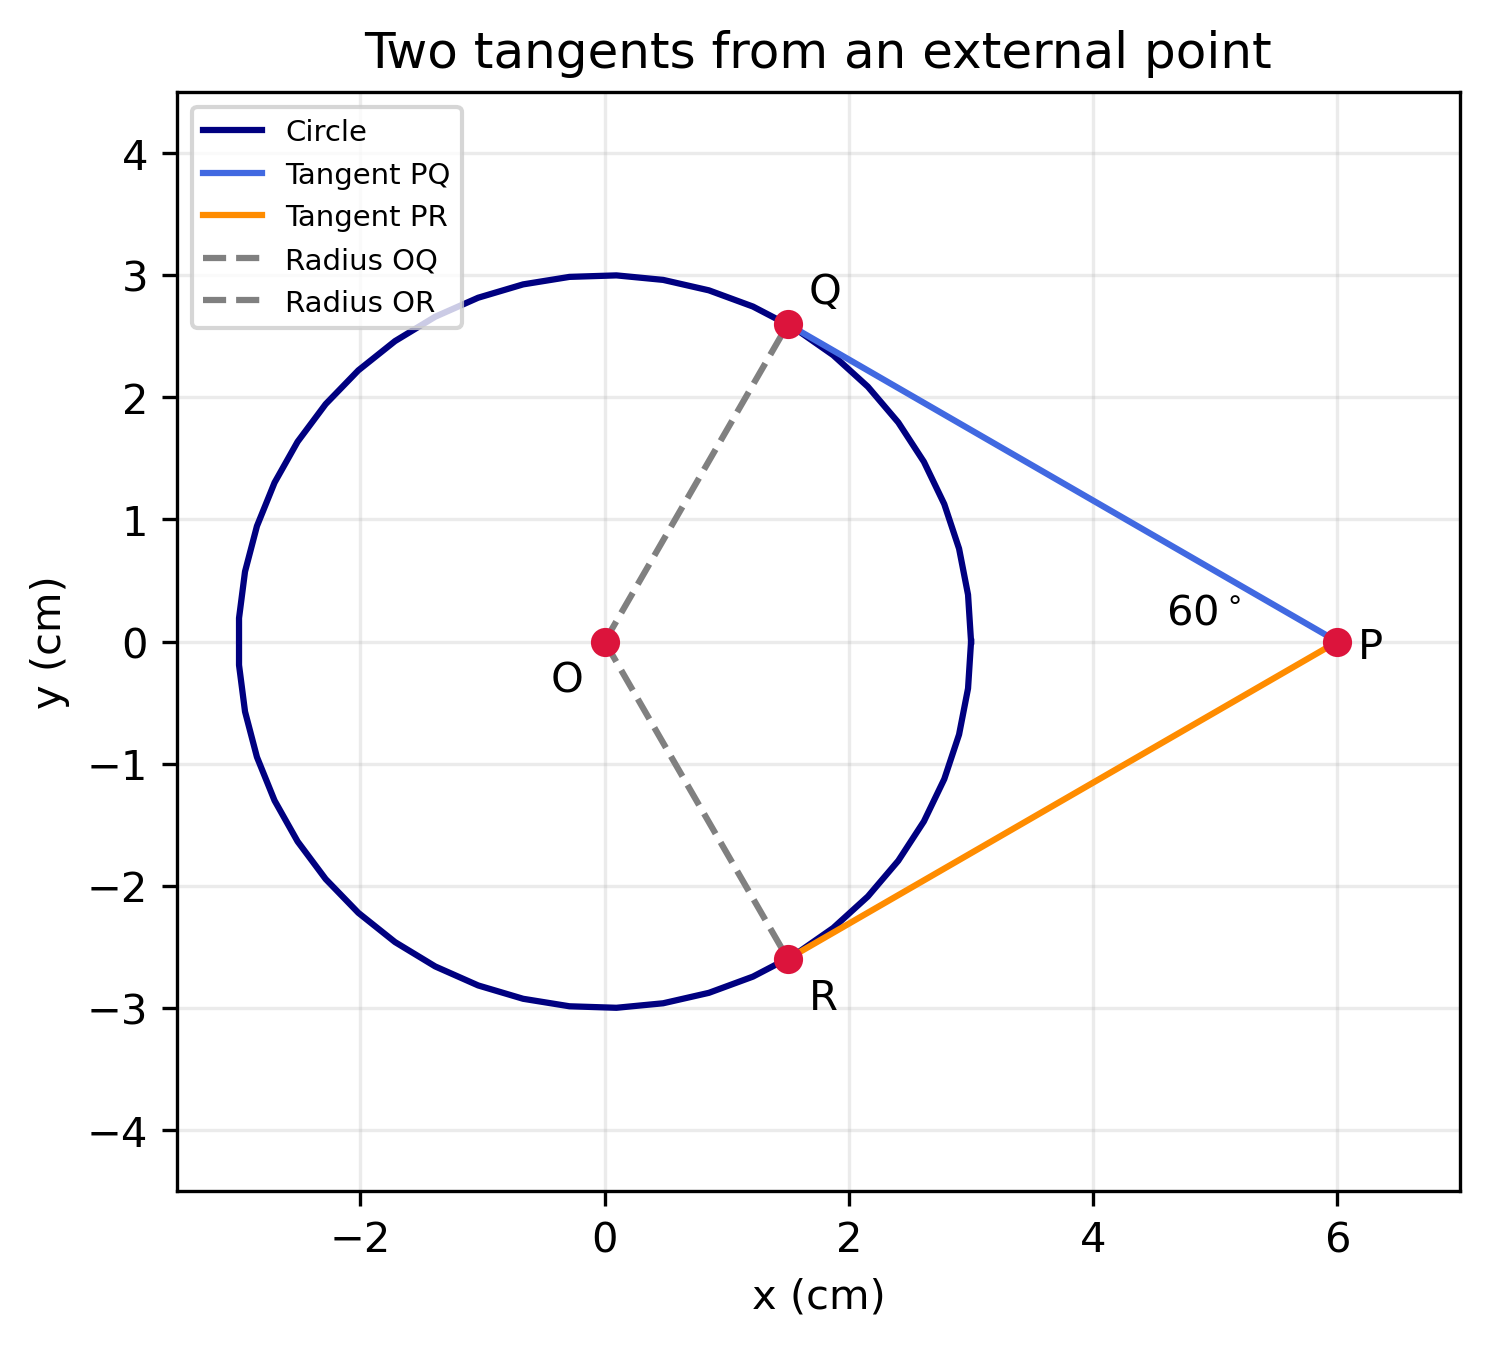
\includegraphics[width=0.47\linewidth]{figs/3.1.2.png}
    \caption{Two equal tangents from $P$ to the circle.}
\end{figure}

\item[3.1.3] In $\triangle DEF$, $AB\parallel EF$. The labelled lengths are $DA=2x$, $AE=3x+1$, $DB=x$, and $BF=2x-\frac12$. Find $x$.

\noindent (A) $0,2$ \hfill (B) $2$ only \hfill (C) $-2$ \hfill (D) $1$

\vspace{0.6em}\par\noindent\textbf{Solution:}

By the Basic Proportionality Theorem,
\[
\frac{2x}{3x+1}=\frac{x}{2x-\frac12},
\]
which gives $x=0$ or $x=2$. Since the labelled lengths must be positive, $x=0$ is invalid. Thus $x=2$, option \textbf{(B)}.

\item[3.1.4] The number $(3\times11\times13+3)$ is:

\noindent (A) prime \hfill (B) divisible by $13$ \hfill (C) composite \hfill (D) odd

\vspace{0.6em}\par\noindent\textbf{Solution:}

The expression is $432$, which is composite. The C program checks each listed property and identifies the correct option, \textbf{(C)}.
\begin{lstlisting}[frame=single, basicstyle=\rmfamily, escapeinside={(*@}{@*)}]
(*@\makebox[\dimexpr\linewidth-2\fboxsep-2\fboxrule\relax][c]{codes/3.1.4.c}@*)
\end{lstlisting}

\item[3.1.5] Two dice are rolled together. Find the probability that the sum of the numbers obtained is divisible by $6$.

\noindent (A) $\frac16$ \hfill (B) $\frac{11}{36}$ \hfill (C) $\frac1{12}$ \hfill (D) $\frac14$

\vspace{0.6em}\par\noindent\textbf{Solution:}

The possible sums divisible by $6$ are $6$ and $12$. They occur in $5+1=6$ of the $36$ equally likely outcomes, so $P=\frac6{36}=\boxed{\frac16}$, option \textbf{(A)}. The simulation uses $500{,}000$ rolls and plots the observed distribution of the sums.
\begin{lstlisting}[frame=single, basicstyle=\rmfamily, escapeinside={(*@}{@*)}]
(*@\makebox[\dimexpr\linewidth-2\fboxsep-2\fboxrule\relax][c]{codes/3.1.5.py}@*)
\end{lstlisting}
\begin{figure}[H]
    \centering
    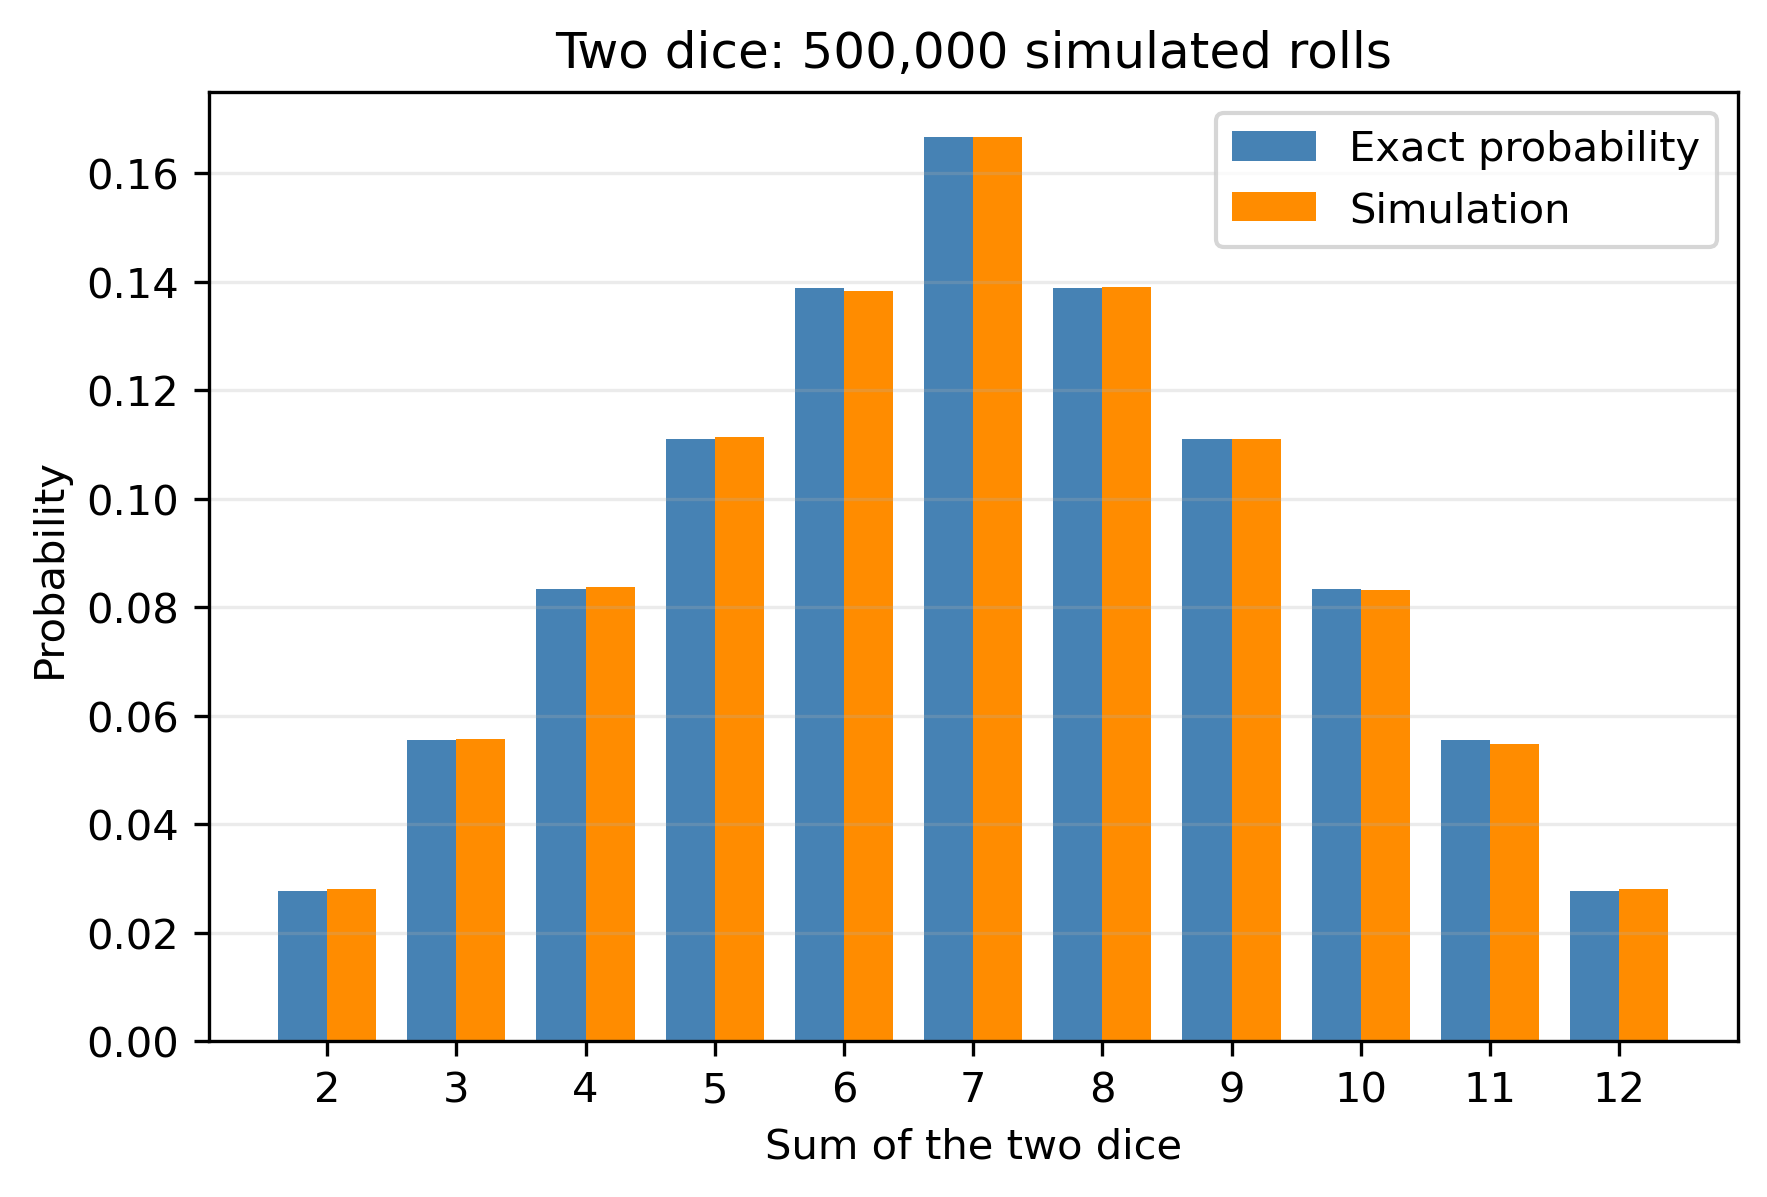
\includegraphics[width=0.50\linewidth]{figs/3.1.5.png}
    \caption{Simulated and exact probability distributions for the sum of two dice.}
\end{figure}

\item[3.1.7] A cone of maximum size is carved out of a solid cube of edge length $\ell$. Find its volume.

\noindent (A) $\frac{\pi\ell^3}{12}$ \hfill (B) $\frac{\pi\ell^3}{3}$ \\
(C) $\ell^3(1-\frac\pi3)$ \hfill (D) $\frac{\pi\ell^3}{8}$

\vspace{0.6em}\par\noindent\textbf{Solution:}

The largest circular base that fits on a face has radius $\ell/2$, and the maximum cone height is $\ell$. Thus $V=\frac13\pi(\ell/2)^2\ell=\boxed{\frac{\pi\ell^3}{12}}$, option \textbf{(A)}. The code searches the feasible radius and height ranges to confirm the maximizing dimensions.
\begin{lstlisting}[frame=single, basicstyle=\rmfamily, escapeinside={(*@}{@*)}]
(*@\makebox[\dimexpr\linewidth-2\fboxsep-2\fboxrule\relax][c]{codes/3.1.7.py}@*)
\end{lstlisting}
\begin{figure}[H]
    \centering
    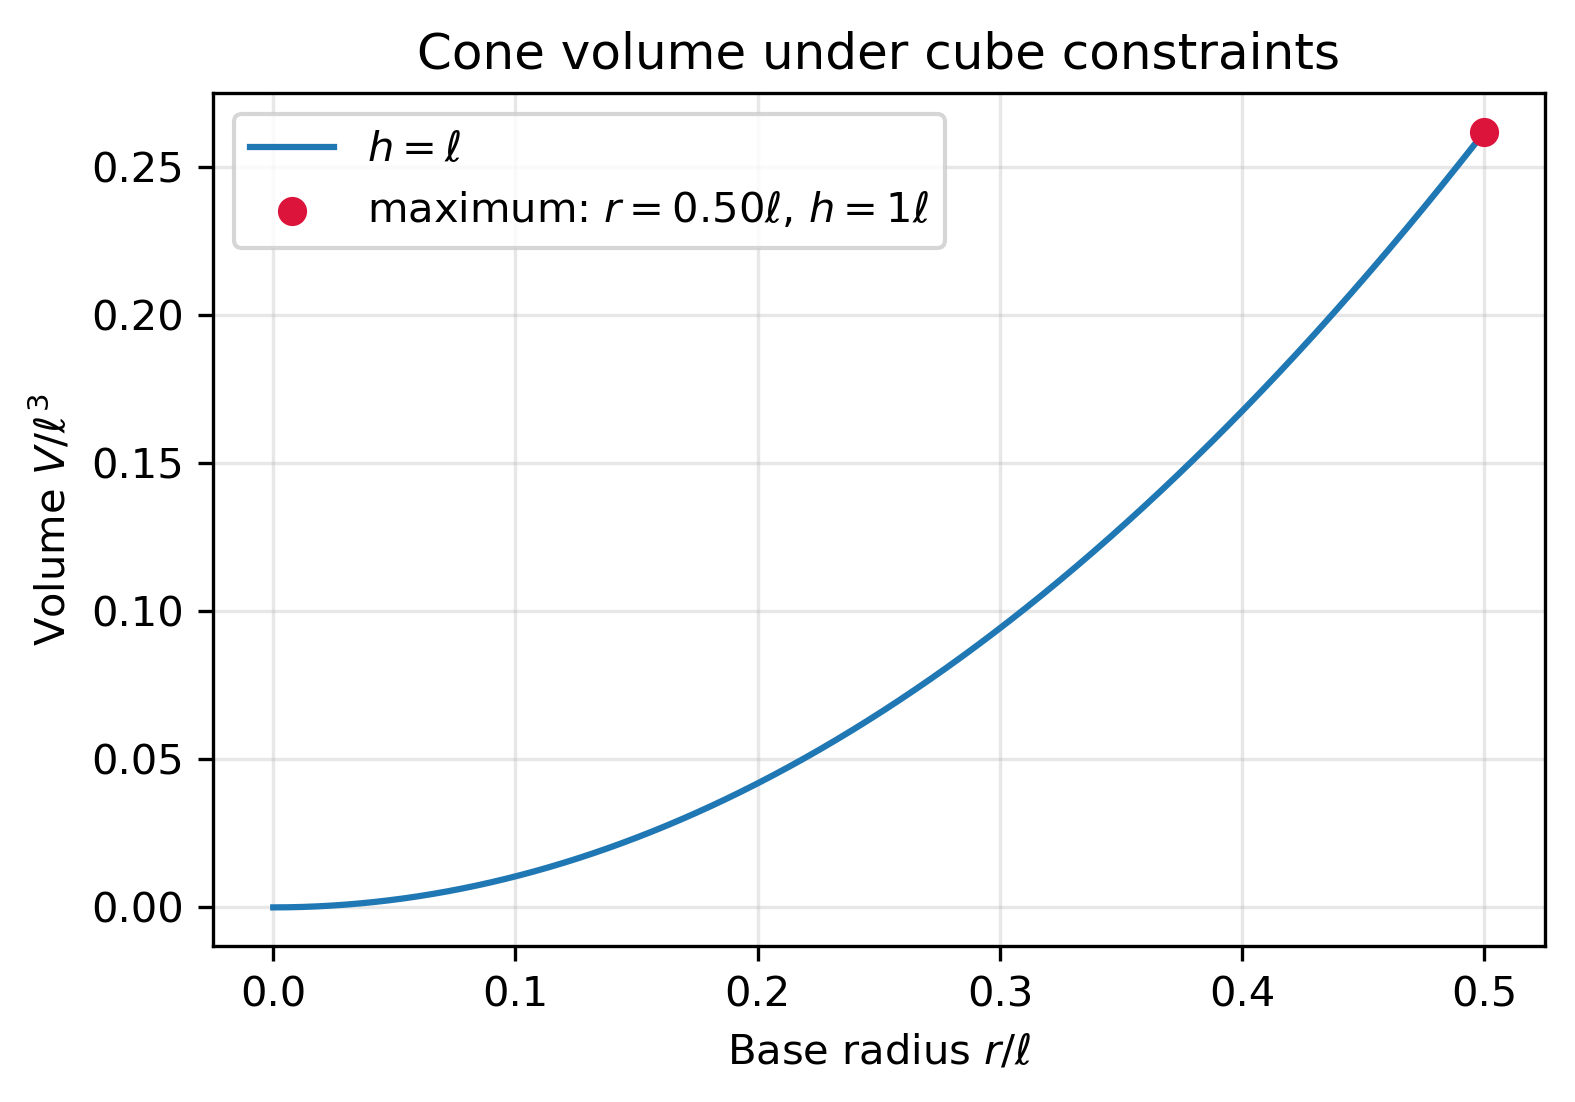
\includegraphics[width=0.45\linewidth]{figs/3.1.7.png}
    \caption{Cone volume as its base radius varies at maximum height.}
\end{figure}

\item[3.1.8] The equation of another line parallel to $2x-6y=7$ is:

\noindent (A) $y=3x-7$ \hfill (B) $2x=9-6y$ \\
(C) $x-3y=7$ \hfill (D) $x=\frac72-3y$

\vspace{0.6em}\par\noindent\textbf{Solution:}

The given line has slope $\frac13$. Only option (C), $y=\frac13x-\frac73$, has the same slope and a different intercept. Hence the answer is \textbf{(C)}. The code plots the given line and all four options.
\begin{lstlisting}[frame=single, basicstyle=\rmfamily, escapeinside={(*@}{@*)}]
(*@\makebox[\dimexpr\linewidth-2\fboxsep-2\fboxrule\relax][c]{codes/3.1.8.py}@*)
\end{lstlisting}
\begin{figure}[H]
    \centering
    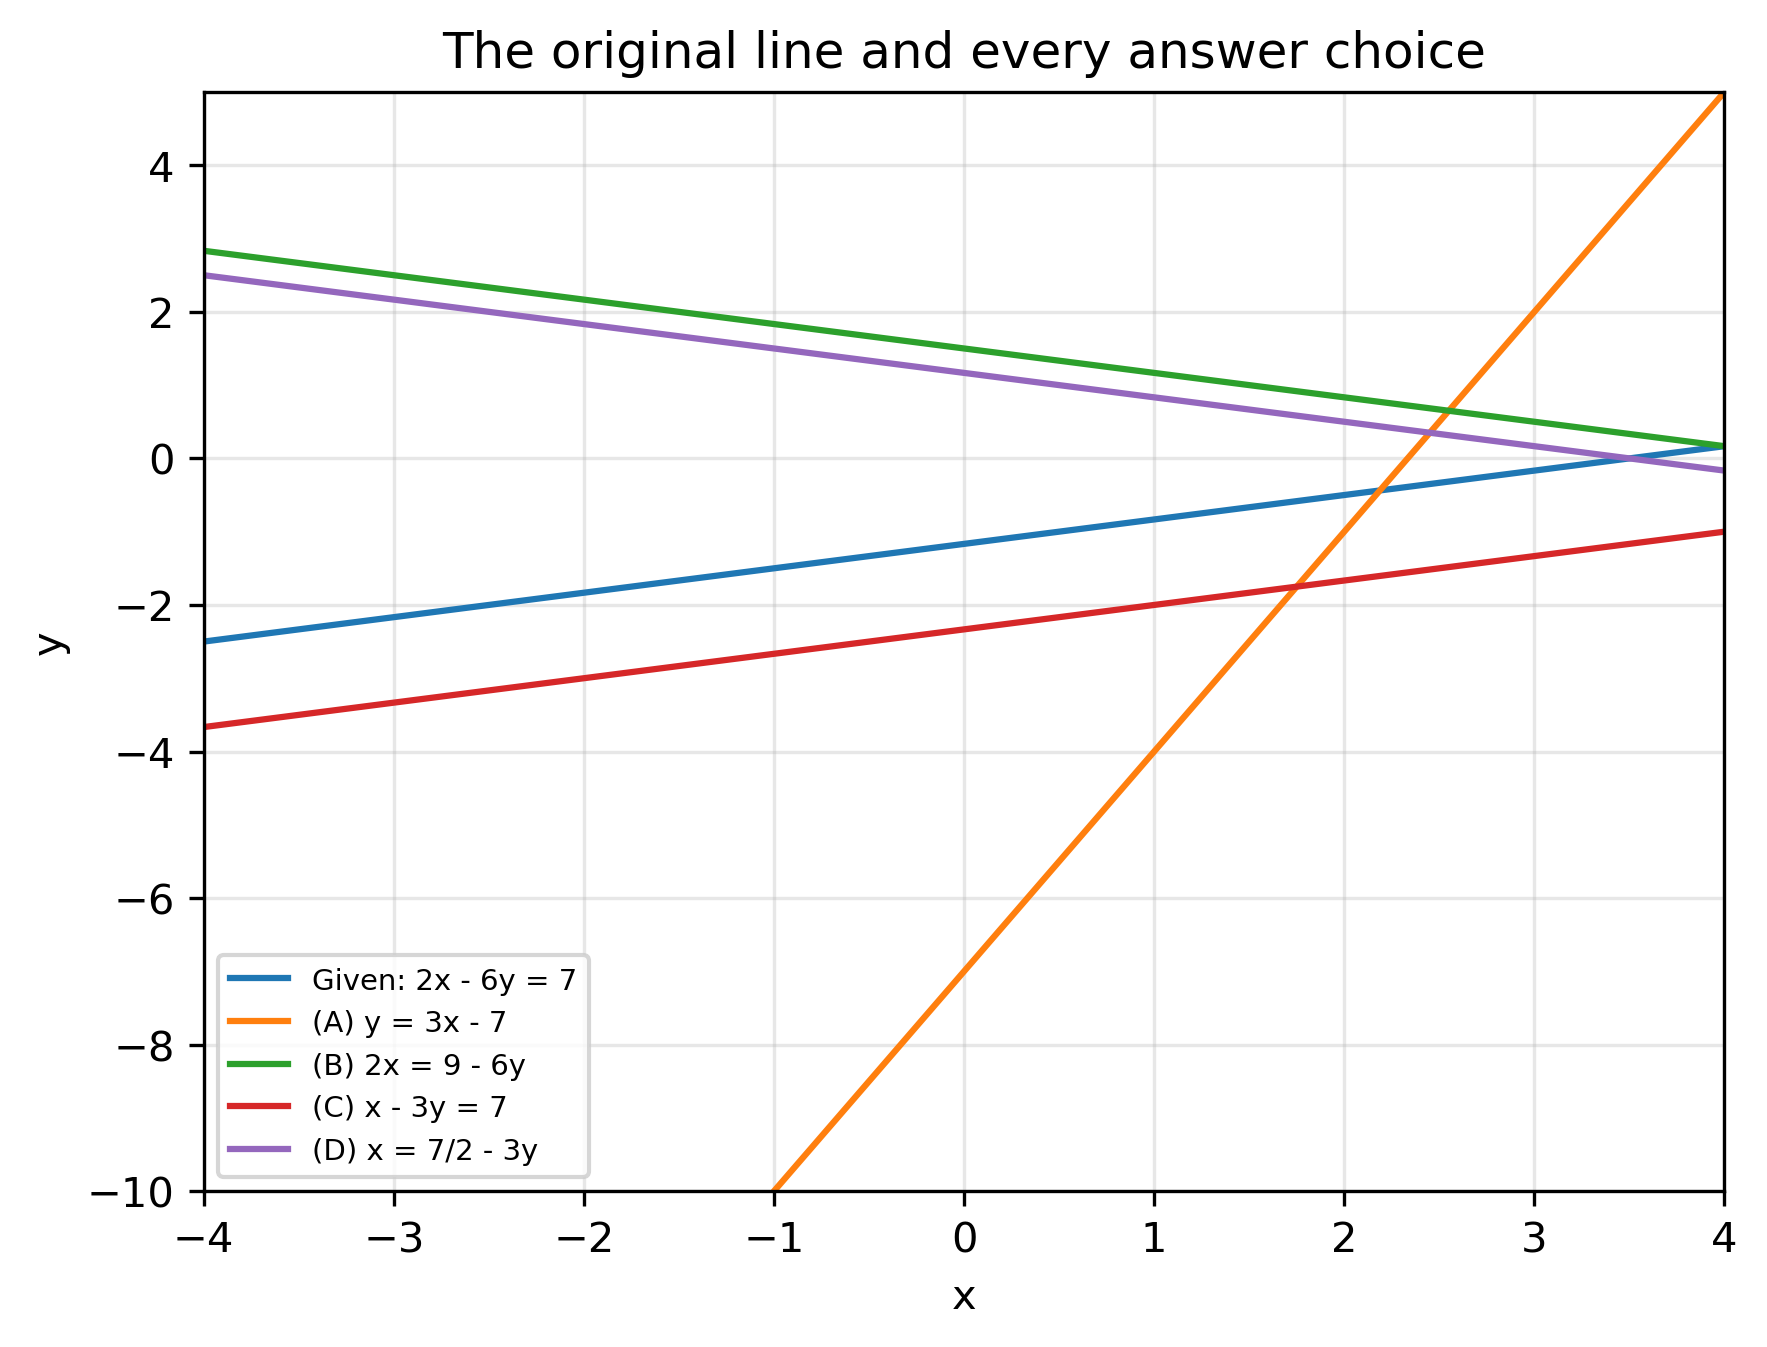
\includegraphics[width=0.57\linewidth]{figs/3.1.8.png}
    \caption{The given line and the four candidate lines.}
\end{figure}

\item[3.1.10] If the roots of $\sqrt3x^2-kx+2\sqrt3=0$ are real and equal, find the value(s) of $k$.

\noindent (A) $\pm\sqrt{24}$ \hfill (B) $0$ \hfill (C) $4$ \hfill (D) $-5$

\vspace{0.6em}\par\noindent\textbf{Solution:}

Equal real roots require a zero discriminant: $k^2-4(\sqrt3)(2\sqrt3)=0$, so $k^2=24$ and $k=\pm\sqrt{24}$. The correct answer is \textbf{(A)}. The code plots both resulting parabolas.
\begin{lstlisting}[frame=single, basicstyle=\rmfamily, escapeinside={(*@}{@*)}]
(*@\makebox[\dimexpr\linewidth-2\fboxsep-2\fboxrule\relax][c]{codes/3.1.10.py}@*)
\end{lstlisting}
\begin{figure}[H]
    \centering
    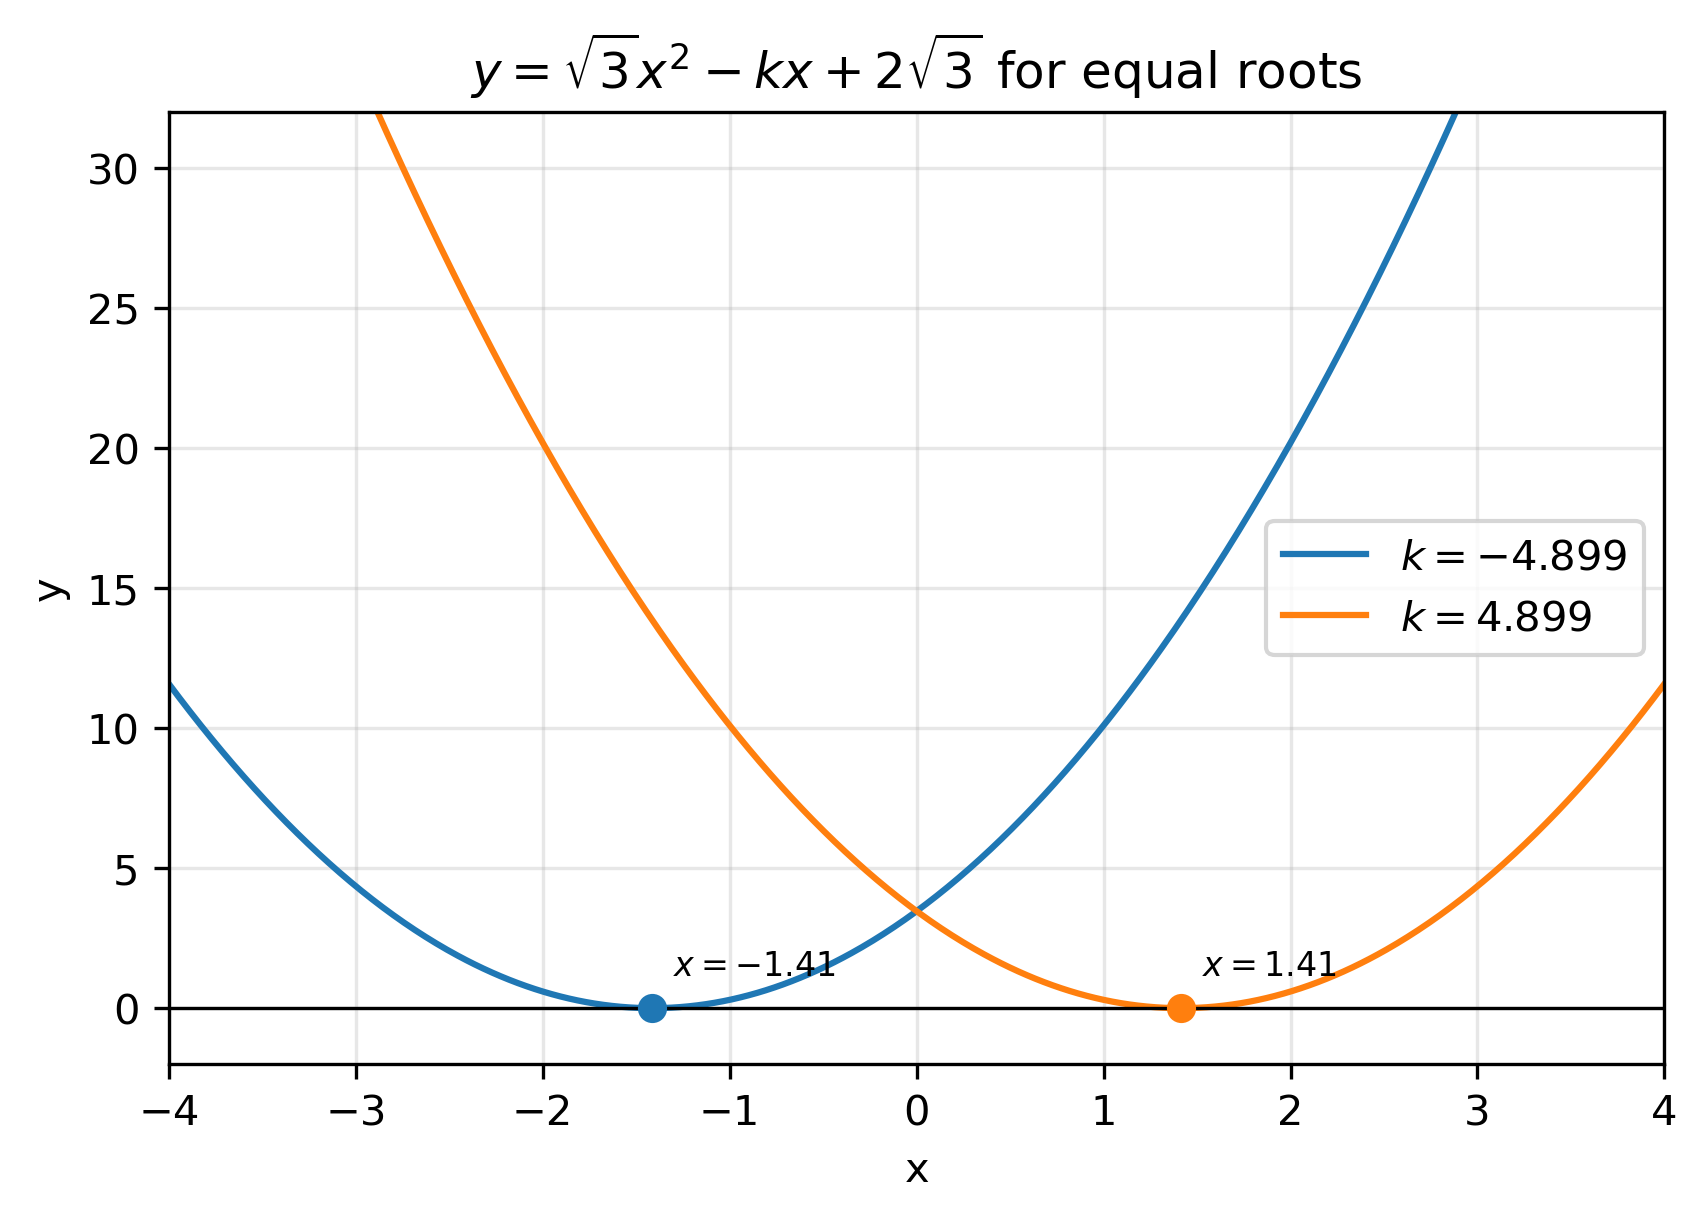
\includegraphics[width=0.52\linewidth]{figs/3.1.10.png}
    \caption{The equal-root parabolas for $k=\pm\sqrt{24}$.}
\end{figure}

\item[3.1.12] A tangent $PT$ is drawn to a circle with centre $O$ and radius $r$. If $\angle POT=45^\circ$, find $OP$.

\noindent (A) $r\sqrt2$ \hfill (B) $\sqrt{2r}$ \hfill (C) $2r$ \hfill (D) $r^2$

\vspace{0.6em}\par\noindent\textbf{Solution:}

Since $OT\perp PT$, $\triangle OTP$ is right-angled at $T$. With $\angle POT=45^\circ$, it is a $45^\circ$-$45^\circ$-$90^\circ$ triangle, so $OP=r\sqrt2$. The answer is \textbf{(A)}. The code draws the circle, tangent, and radius and calculates $OP$.
\begin{lstlisting}[frame=single, basicstyle=\rmfamily, escapeinside={(*@}{@*)}]
(*@\makebox[\dimexpr\linewidth-2\fboxsep-2\fboxrule\relax][c]{codes/3.1.12.py}@*)
\end{lstlisting}
\begin{figure}[H]
    \centering
    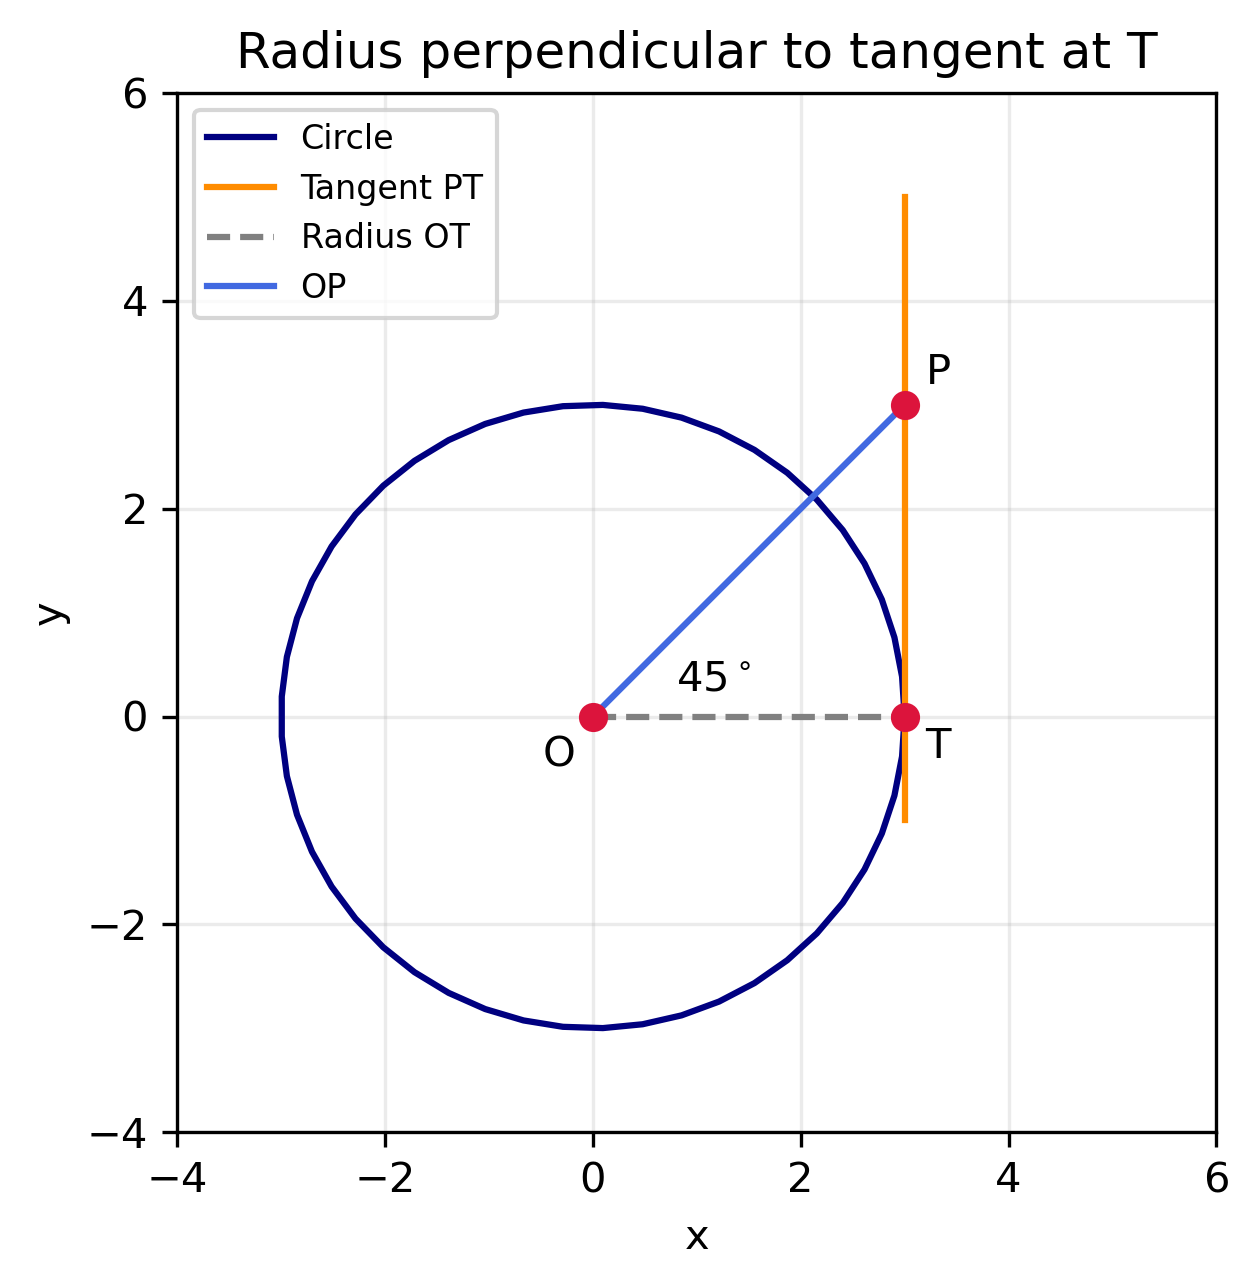
\includegraphics[width=0.48\linewidth]{figs/3.1.12.png}
    \caption{Tangent $PT$ perpendicular to radius $OT$.}
\end{figure}

\item[3.1.14] The sum and product of the zeroes of a quadratic polynomial $p(x)$ are $-\frac13$ and $2$ respectively. The polynomial $p(x)$ is:

\noindent (A) $3x^2-x+6$ \hfill (B) $x^2+\frac13x-2$ \\
(C) $3x^2-x+2$ \hfill (D) $-3x^2-x-6$

\vspace{0.6em}\par\noindent\textbf{Solution:}

For $ax^2+bx+c$, the sum and product of zeroes are $-b/a$ and $c/a$. Option (D) gives $-1/3$ and $2$, so it is correct. Its graph has no real zeroes, consistent with its negative discriminant.
\begin{lstlisting}[frame=single, basicstyle=\rmfamily, escapeinside={(*@}{@*)}]
(*@\makebox[\dimexpr\linewidth-2\fboxsep-2\fboxrule\relax][c]{codes/3.1.14.py}@*)
\end{lstlisting}
\begin{figure}[H]
    \centering
    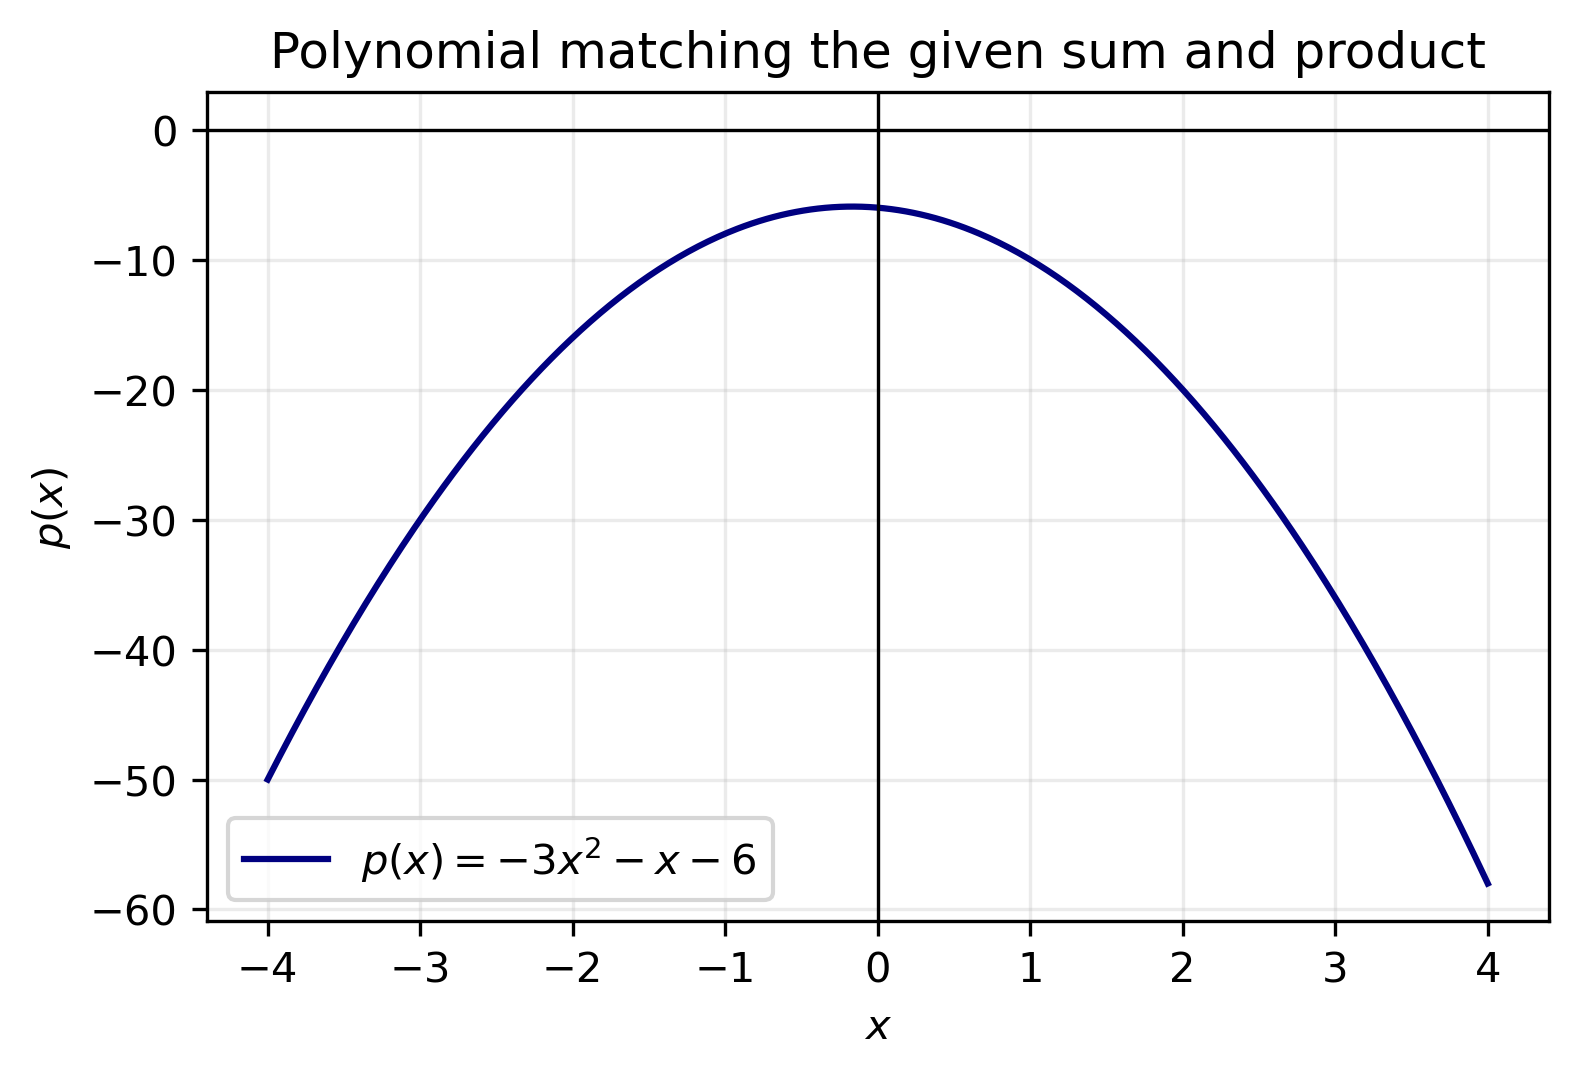
\includegraphics[width=0.51\linewidth]{figs/3.1.14.png}
    \caption{Graph of the polynomial in option (D).}
\end{figure}

\item[3.1.17] In the figure, $\triangle ABC$ is equilateral and $AD$ is a median joining $A(0,\frac{5\sqrt3}{2})$ and $D(0,0)$. Find coordinates of $B$ and $C$ in that order.

\noindent (A) $(-5,0),(5,0)$ \hfill (B) $(-\frac52,0),(\frac52,0)$ \\
(C) $(-10,0),(10,0)$ \hfill (D) $(-5\sqrt3,0),(5\sqrt3,0)$

\vspace{0.6em}\par\noindent\textbf{Solution:}

The altitude is $AD=5\sqrt3/2$. For an equilateral triangle, $h=(\sqrt3/2)s$, so the side is $s=5$. Since $D$ is the midpoint of $BC$, $B=(-5/2,0)$ and $C=(5/2,0)$, option \textbf{(B)}. The code uses the given coordinates to construct the triangle and median.
\begin{lstlisting}[frame=single, basicstyle=\rmfamily, escapeinside={(*@}{@*)}]
(*@\makebox[\dimexpr\linewidth-2\fboxsep-2\fboxrule\relax][c]{codes/3.1.17.py}@*)
\end{lstlisting}
\begin{figure}[H]
    \centering
    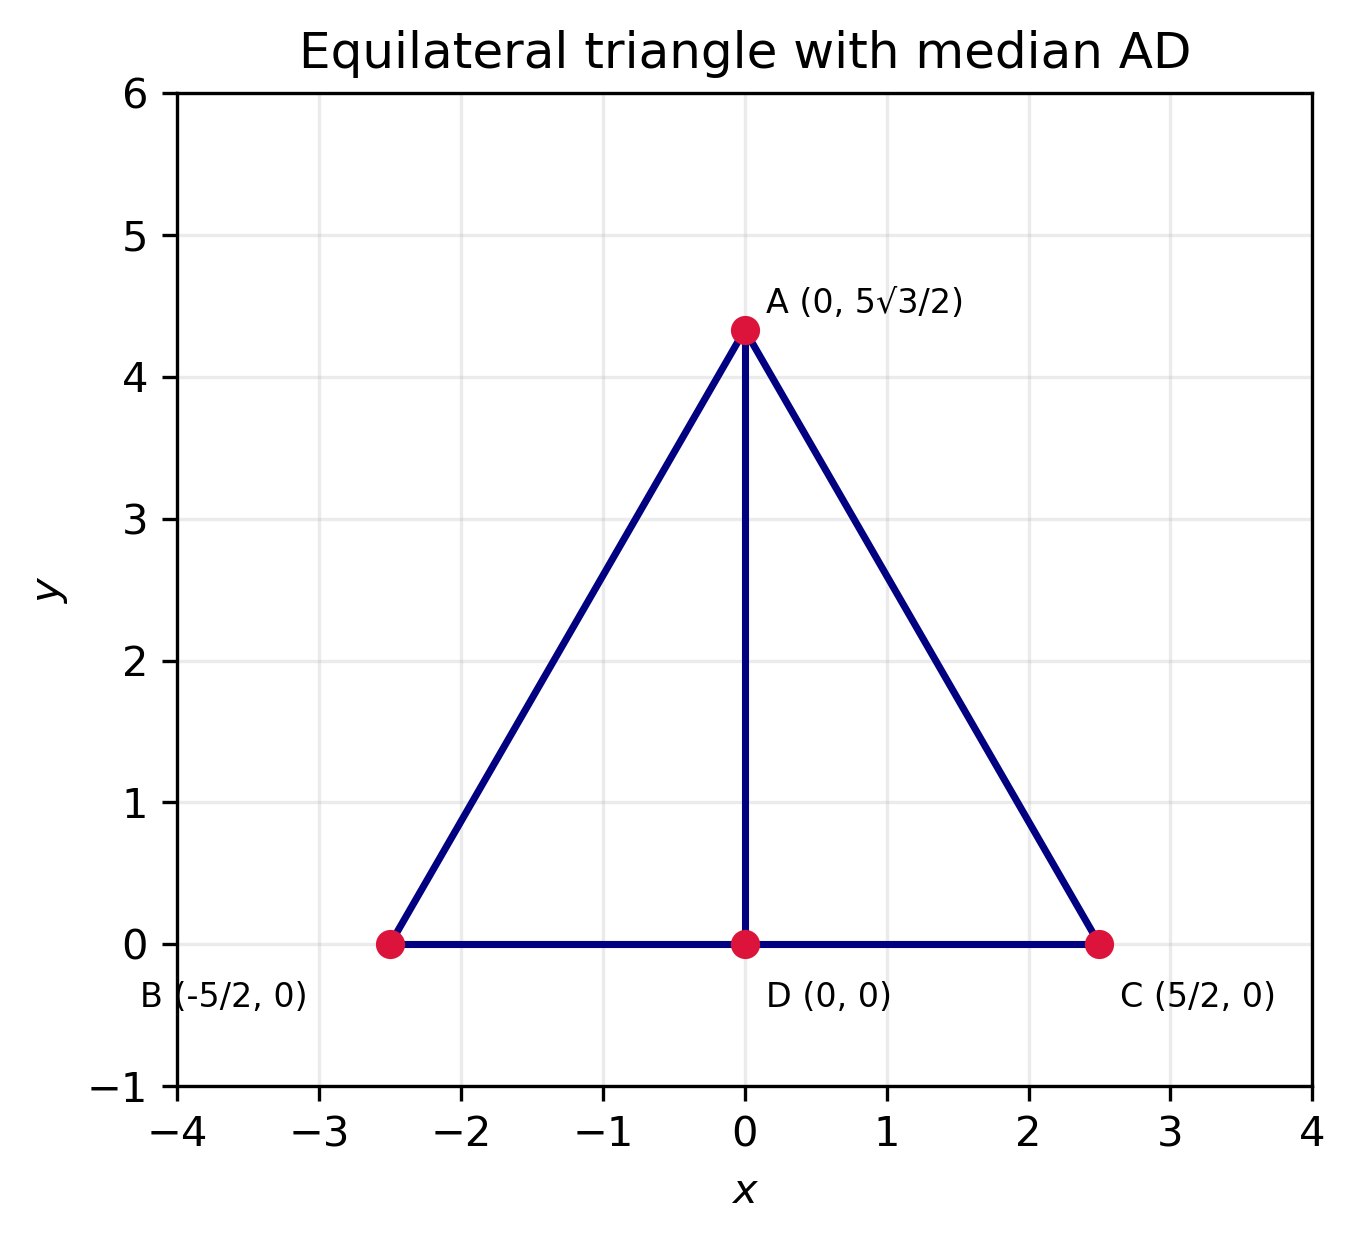
\includegraphics[width=0.48\linewidth]{figs/3.1.17.png}
    \caption{Equilateral triangle $ABC$ and median $AD$.}
\end{figure}

\item[3.1.21] Find the length of a plank that can measure $4$ m $20$ cm and $5$ m $4$ cm exactly, in the least time.

\vspace{0.6em}\par\noindent\textbf{Solution:}

The greatest possible plank length is the HCF of $420$ cm and $504$ cm, which is $84$ cm. The C program applies Euclid's algorithm.
\begin{lstlisting}[frame=single, basicstyle=\rmfamily, escapeinside={(*@}{@*)}]
(*@\makebox[\dimexpr\linewidth-2\fboxsep-2\fboxrule\relax][c]{codes/3.1.21.c}@*)
\end{lstlisting}

\item[3.1.23] Diagonals $AC$ and $BD$ of square $ABCD$ intersect at $P$. Coordinates of $B$ and $D$ are $(9,-2)$ and $(1,6)$ respectively. (i) Find coordinates of $P$. (ii) Find the side length of the square.

\vspace{0.6em}\par\noindent\textbf{Solution:}

The diagonals bisect each other, so $P$ is the midpoint of $BD$: $P=(5,2)$. The diagonal length is $BD=\sqrt{8^2+(-8)^2}=8\sqrt2$, hence the square's side is $BD/\sqrt2=8$. The code plots the square and its diagonals.
\begin{lstlisting}[frame=single, basicstyle=\rmfamily, escapeinside={(*@}{@*)}]
(*@\makebox[\dimexpr\linewidth-2\fboxsep-2\fboxrule\relax][c]{codes/3.1.23.py}@*)
\end{lstlisting}
\begin{figure}[H]
    \centering
    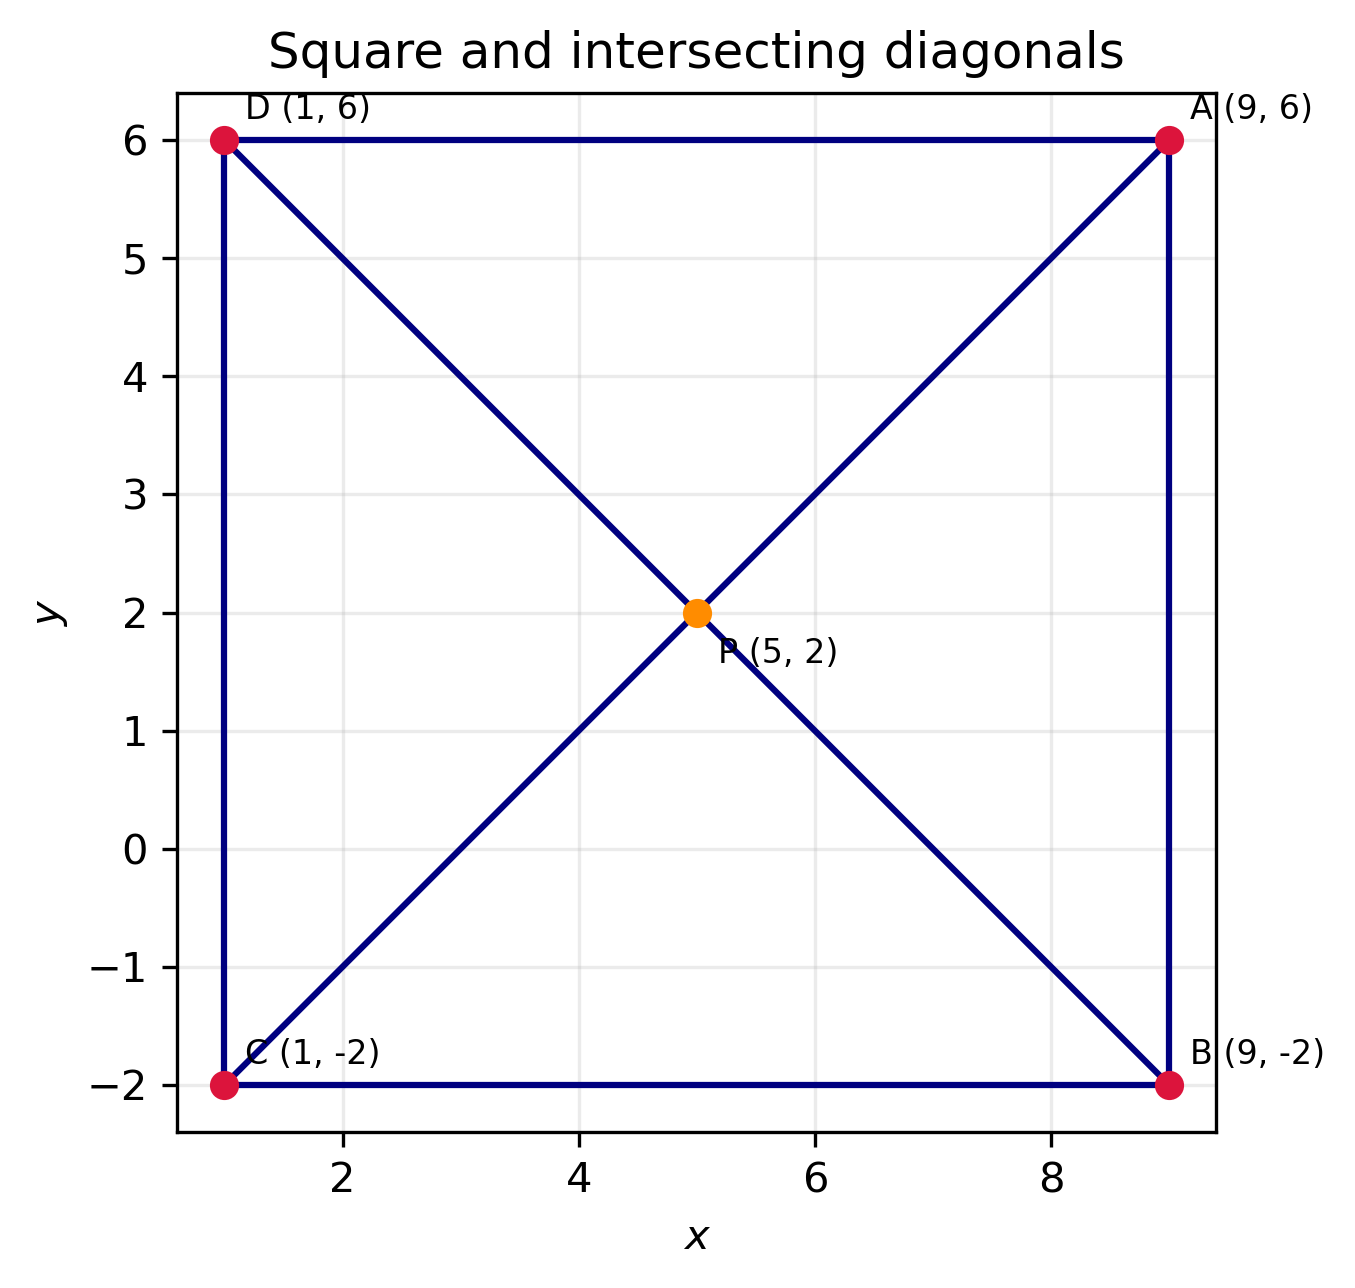
\includegraphics[width=0.49\linewidth]{figs/3.1.23.png}
    \caption{Square $ABCD$ and diagonals meeting at $P$.}
\end{figure}

\item[3.1.27] A chord $AB$ of a circle of radius $7$ cm subtends an angle of $120^\circ$ at the centre. Find (i) the perimeter of major sector $OACB$, and (ii) the area of the shaded segment if $[\triangle OAB]=21.2$ cm$^2$.

\vspace{0.6em}\par\noindent\textbf{Solution:}

The major arc is $240^\circ$, so the major-sector perimeter is $14+\frac{240}{360}(14\pi)=14+\frac{28\pi}{3}\approx43.32$ cm. The shaded minor segment has area $\frac{120}{360}\pi(7)^2-21.2=\frac{49\pi}{3}-21.2\approx30.11$ cm$^2$. The code draws and shades the segment and calculates both values.
\begin{lstlisting}[frame=single, basicstyle=\rmfamily, escapeinside={(*@}{@*)}]
(*@\makebox[\dimexpr\linewidth-2\fboxsep-2\fboxrule\relax][c]{codes/3.1.27.py}@*)
\end{lstlisting}
\begin{figure}[H]
    \centering
    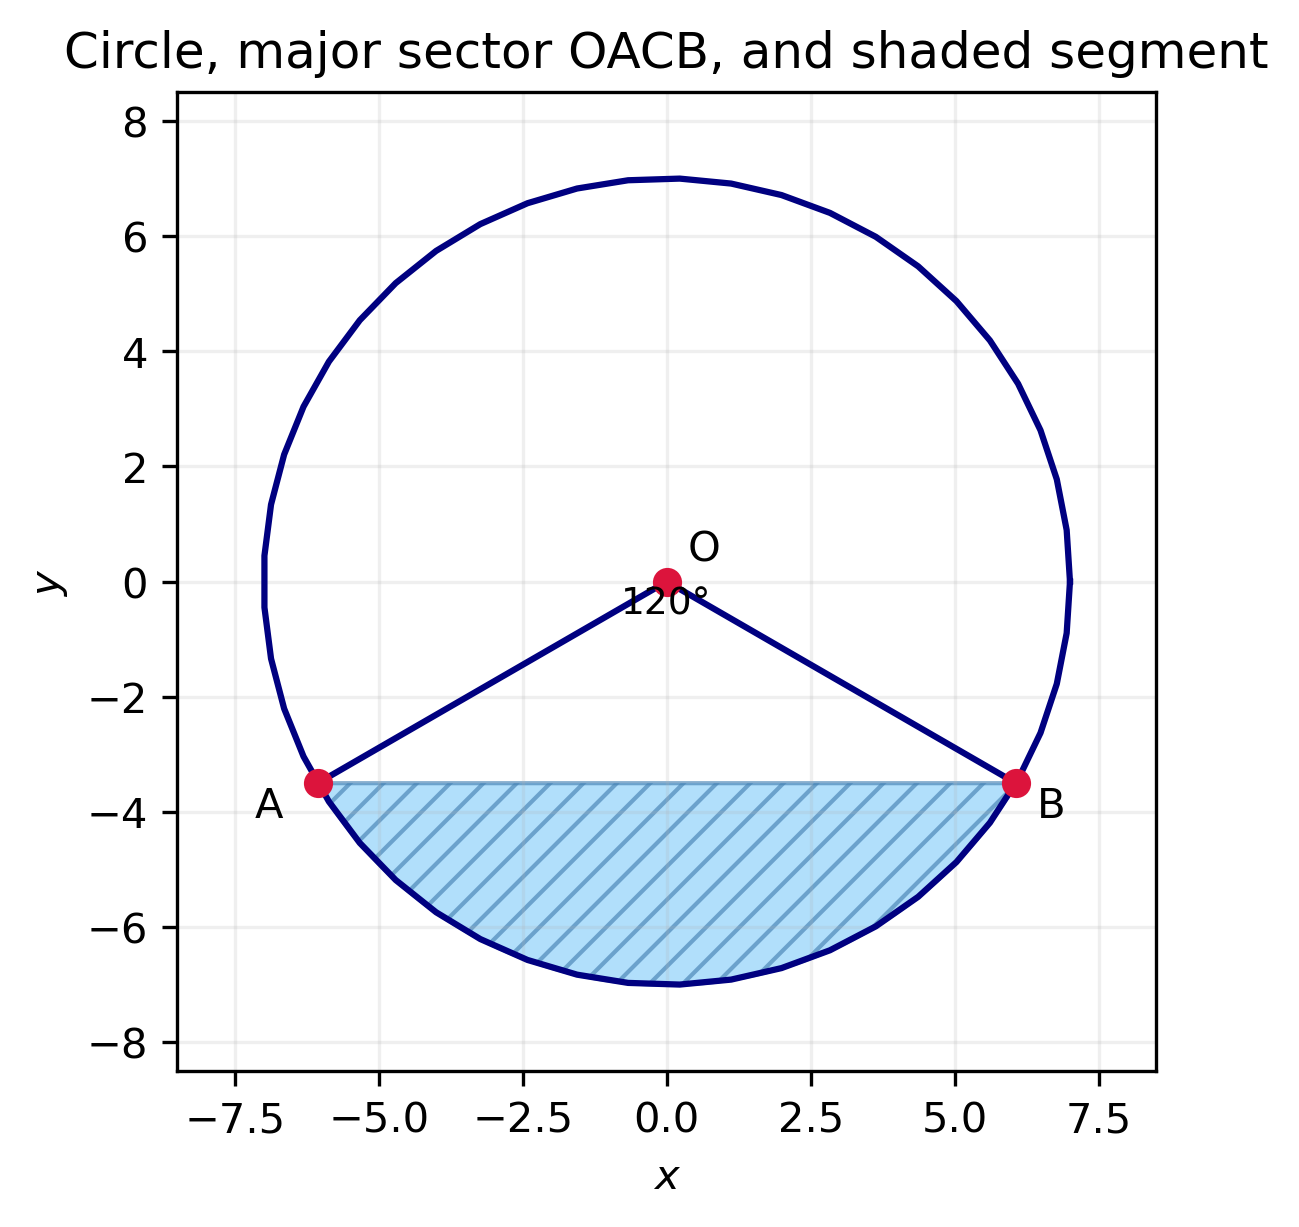
\includegraphics[width=0.47\linewidth]{figs/3.1.27.png}
    \caption{Major sector and shaded minor segment.}
\end{figure}

\item[3.1.30] A point $P(x,7)$ divides the line segment joining $A(-5,4)$ and $B(7,9)$ in a certain ratio. Find the ratio and hence find $x$.

\vspace{0.6em}\par\noindent\textbf{Solution:}

The vertical changes give $AP:PB=(7-4):(9-7)=3:2$. By the section formula, $x=\frac{3(7)+2(-5)}{3+2}=\frac{11}{5}$. The code plots $A$, $P$, and $B$.
\begin{lstlisting}[frame=single, basicstyle=\rmfamily, escapeinside={(*@}{@*)}]
(*@\makebox[\dimexpr\linewidth-2\fboxsep-2\fboxrule\relax][c]{codes/3.1.30.py}@*)
\end{lstlisting}
\begin{figure}[H]
    \centering
    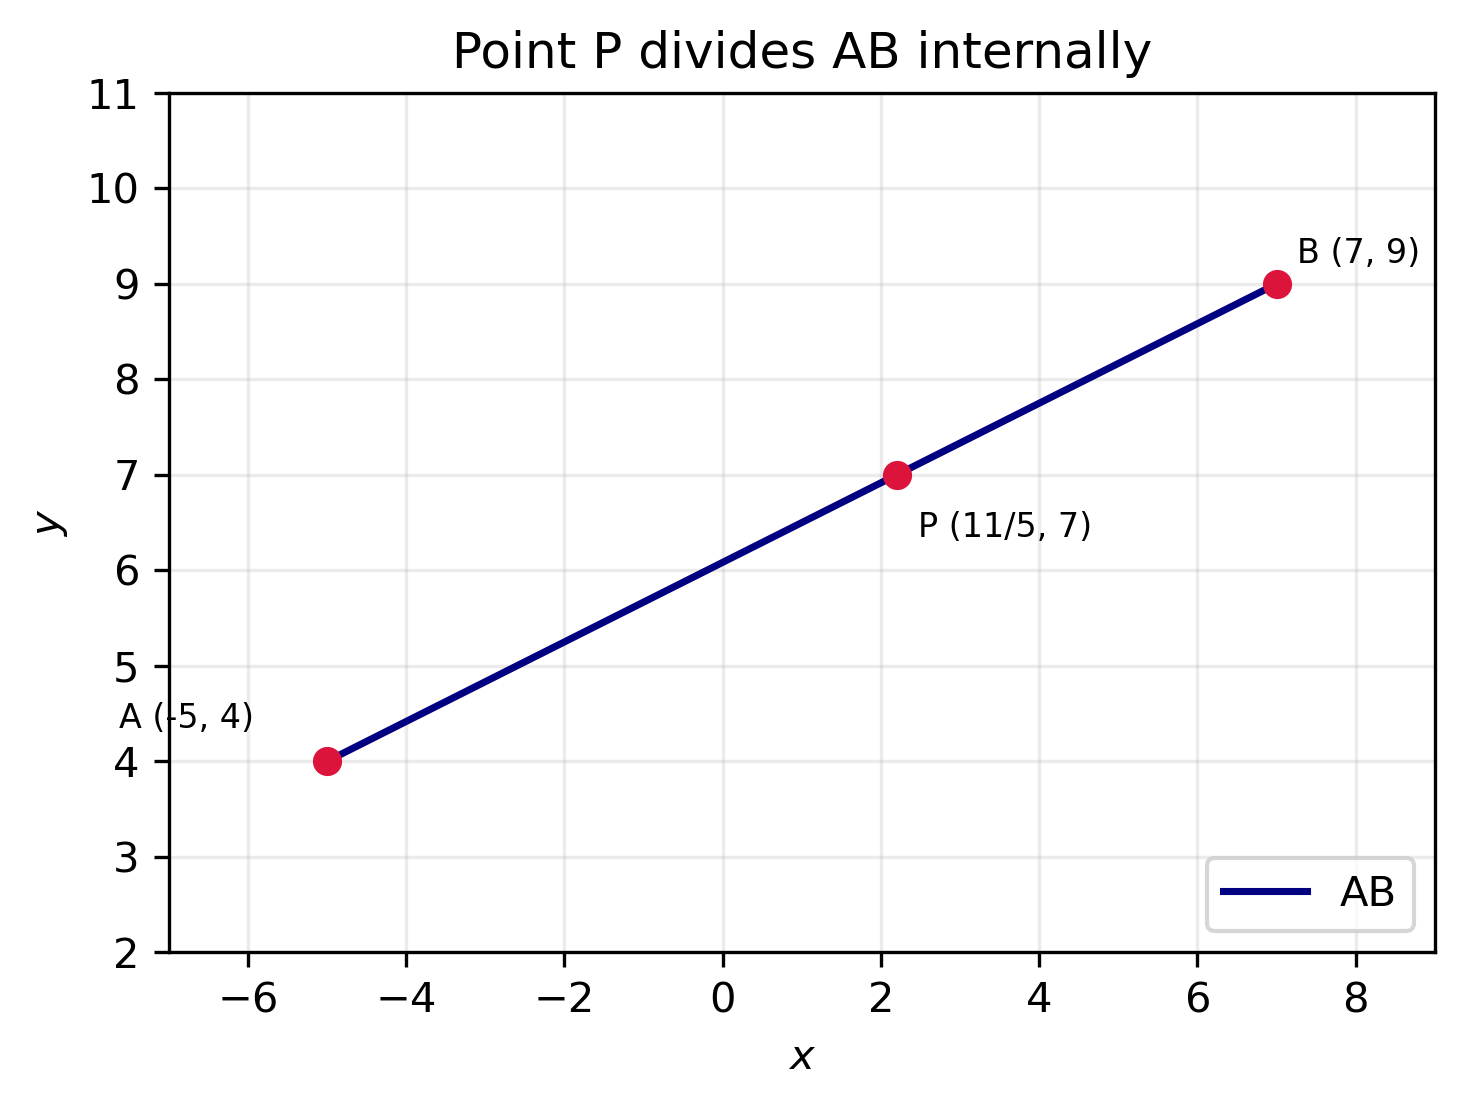
\includegraphics[width=0.52\linewidth]{figs/3.1.30.png}
    \caption{Point $P$ divides $AB$ internally in the ratio $3:2$.}
\end{figure}

\item[3.1.31.2] In the given figure, $PA$ is tangent to the circle with centre $O$, $OA=10$ cm, $AB=8$ cm, and $AB\perp OP$. Find $PB$.

\vspace{0.6em}\par\noindent\textbf{Solution:}

In right triangle $OAB$, $OB=\sqrt{10^2-8^2}=6$ cm. Let $PB=t$. Since $PA$ is tangent, $\triangle OAP$ is right-angled at $A$; also $\triangle PAB$ is right-angled at $B$. Thus $t^2+8^2=(t+6)^2-10^2$, giving $t=\frac{32}{3}$ cm. The code constructs this configuration and computes the length.
\begin{lstlisting}[frame=single, basicstyle=\rmfamily, escapeinside={(*@}{@*)}]
(*@\makebox[\dimexpr\linewidth-2\fboxsep-2\fboxrule\relax][c]{codes/3.1.31.2.py}@*)
\end{lstlisting}
\begin{figure}[H]
    \centering
    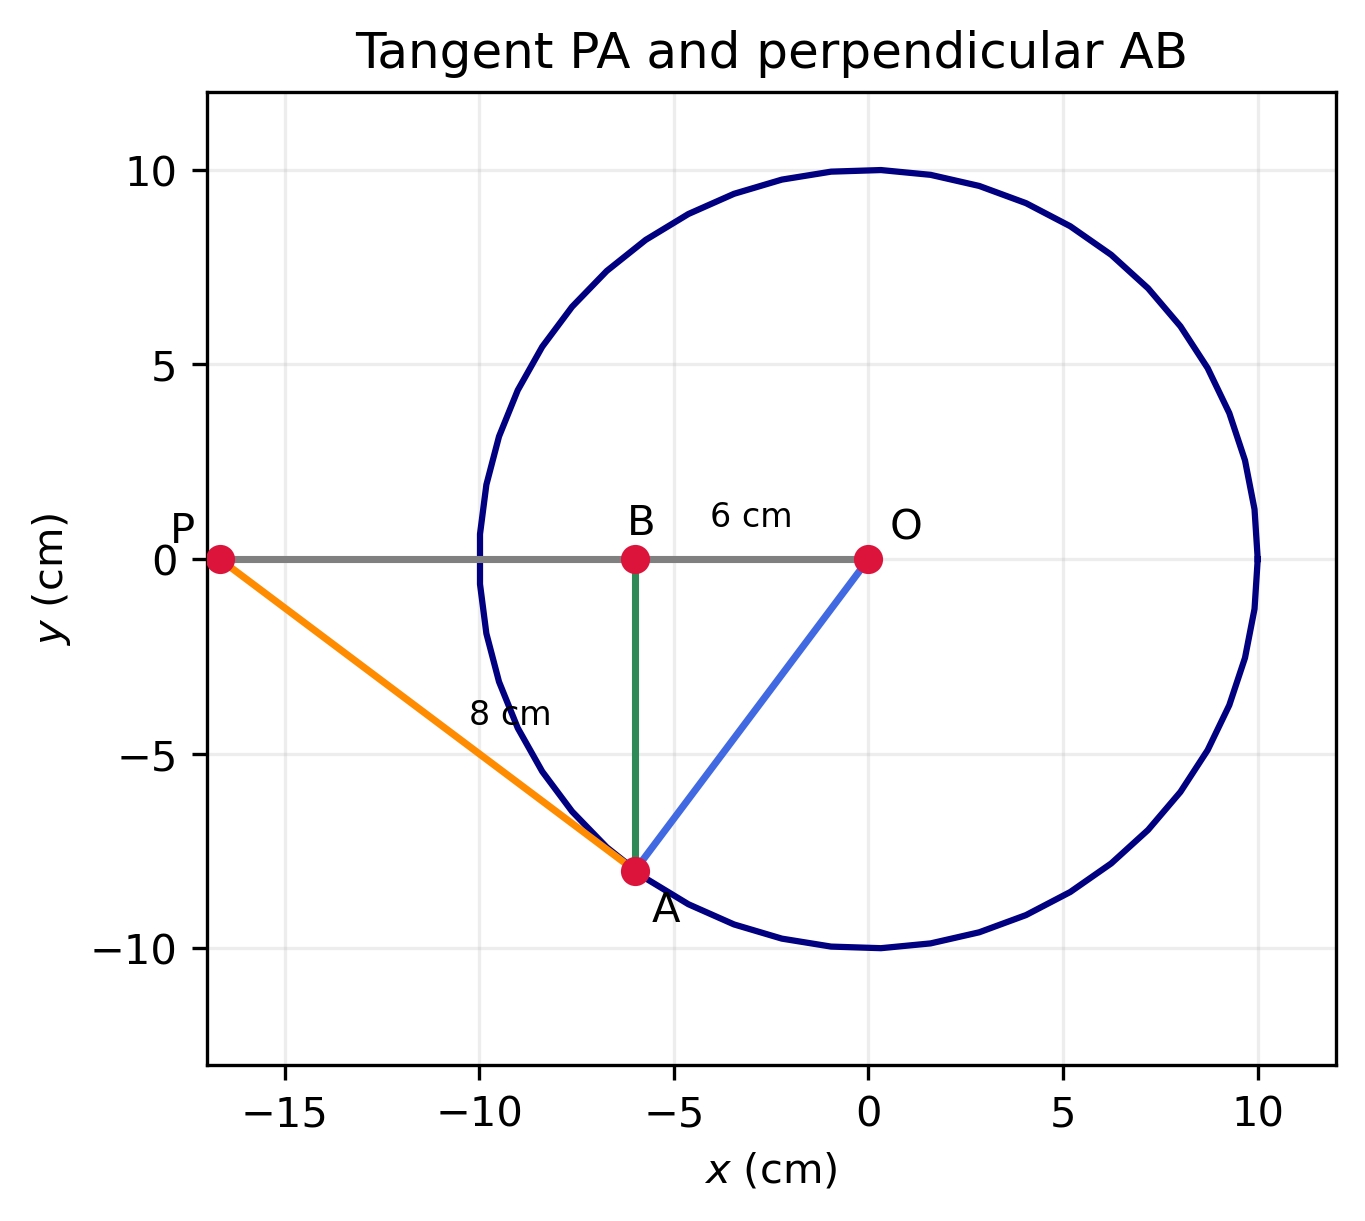
\includegraphics[width=0.50\linewidth]{figs/3.1.31.2.png}
    \caption{Tangent $PA$ and perpendicular segment $AB$.}
\end{figure}

\item[3.1.33] In $\triangle ABC$, $AD$ is a median. $X$ lies on $AD$ with $AX:XD=2:3$. $BX$ is extended to meet $AC$ at $Y$. Prove that $BX=4XY$.

\vspace{0.6em}\par\noindent\textbf{Solution:}

Use coordinates $B=(0,0)$, $C=(2,0)$, and $A=(u,v)$, so $D=(1,0)$. From $AX:XD=2:3$, $X=(3A+2D)/5$. Let $Y=B+t(X-B)$ lie on $AC$. Equating coordinates gives $t=5/4$, so $BY=(5/4)BX$ and $XY=BY-BX=BX/4$. Therefore $BX=4XY$. The code draws a representative triangle and verifies the ratio numerically.
\begin{lstlisting}[frame=single, basicstyle=\rmfamily, escapeinside={(*@}{@*)}]
(*@\makebox[\dimexpr\linewidth-2\fboxsep-2\fboxrule\relax][c]{codes/3.1.33.py}@*)
\end{lstlisting}
\begin{figure}[H]
    \centering
    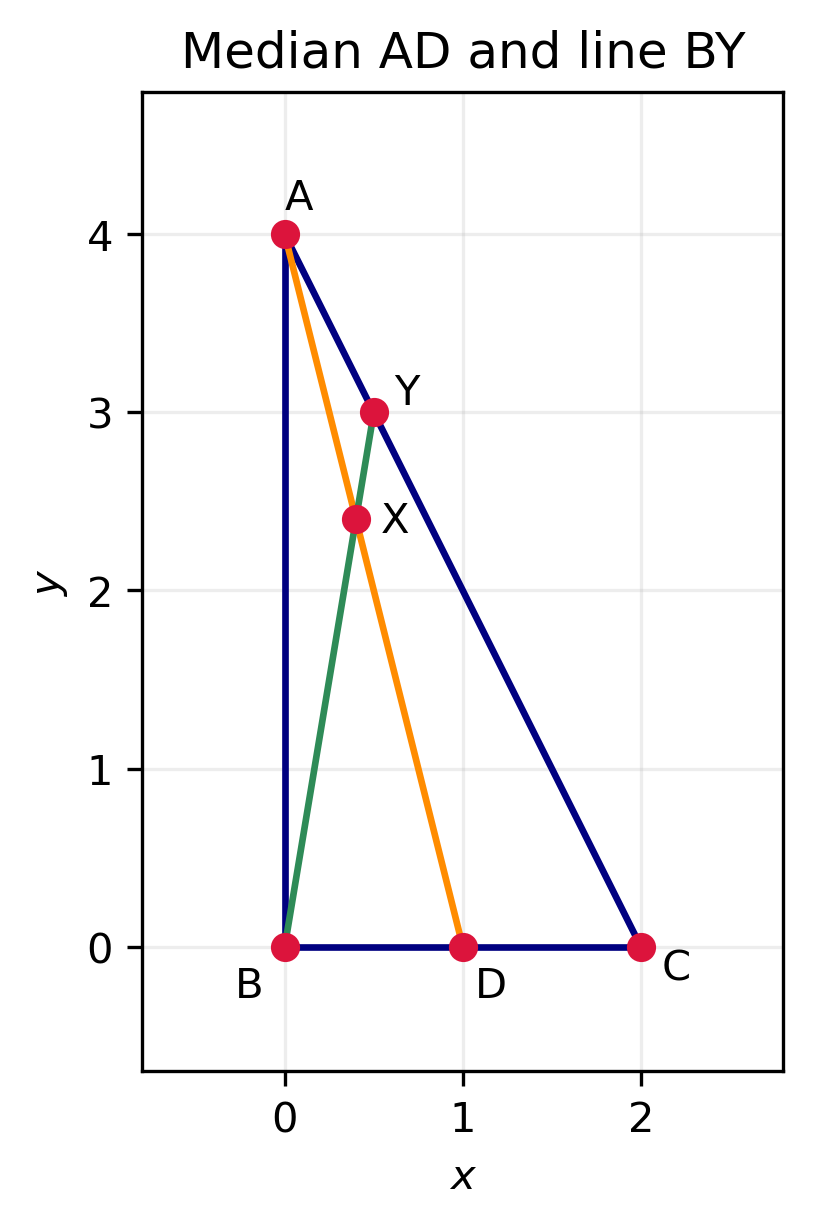
\includegraphics[width=0.47\linewidth]{figs/3.1.33.png}
    \caption{Median $AD$ and the transversal $BY$.}
\end{figure}

\item[3.1.34.1] Solve graphically: $x-2y=3$, $3x-8y=7$.

\vspace{0.6em}\par\noindent\textbf{Solution:}

The two lines intersect at $(5,1)$, so the solution is $x=5$, $y=1$. The code plots both lines and marks their intersection; it uses the CoordGeo line-intersection function to calculate the point.
\begin{lstlisting}[frame=single, basicstyle=\rmfamily, escapeinside={(*@}{@*)}]
(*@\makebox[\dimexpr\linewidth-2\fboxsep-2\fboxrule\relax][c]{codes/3.1.34.1.py}@*)
\end{lstlisting}
\begin{figure}[H]
    \centering
    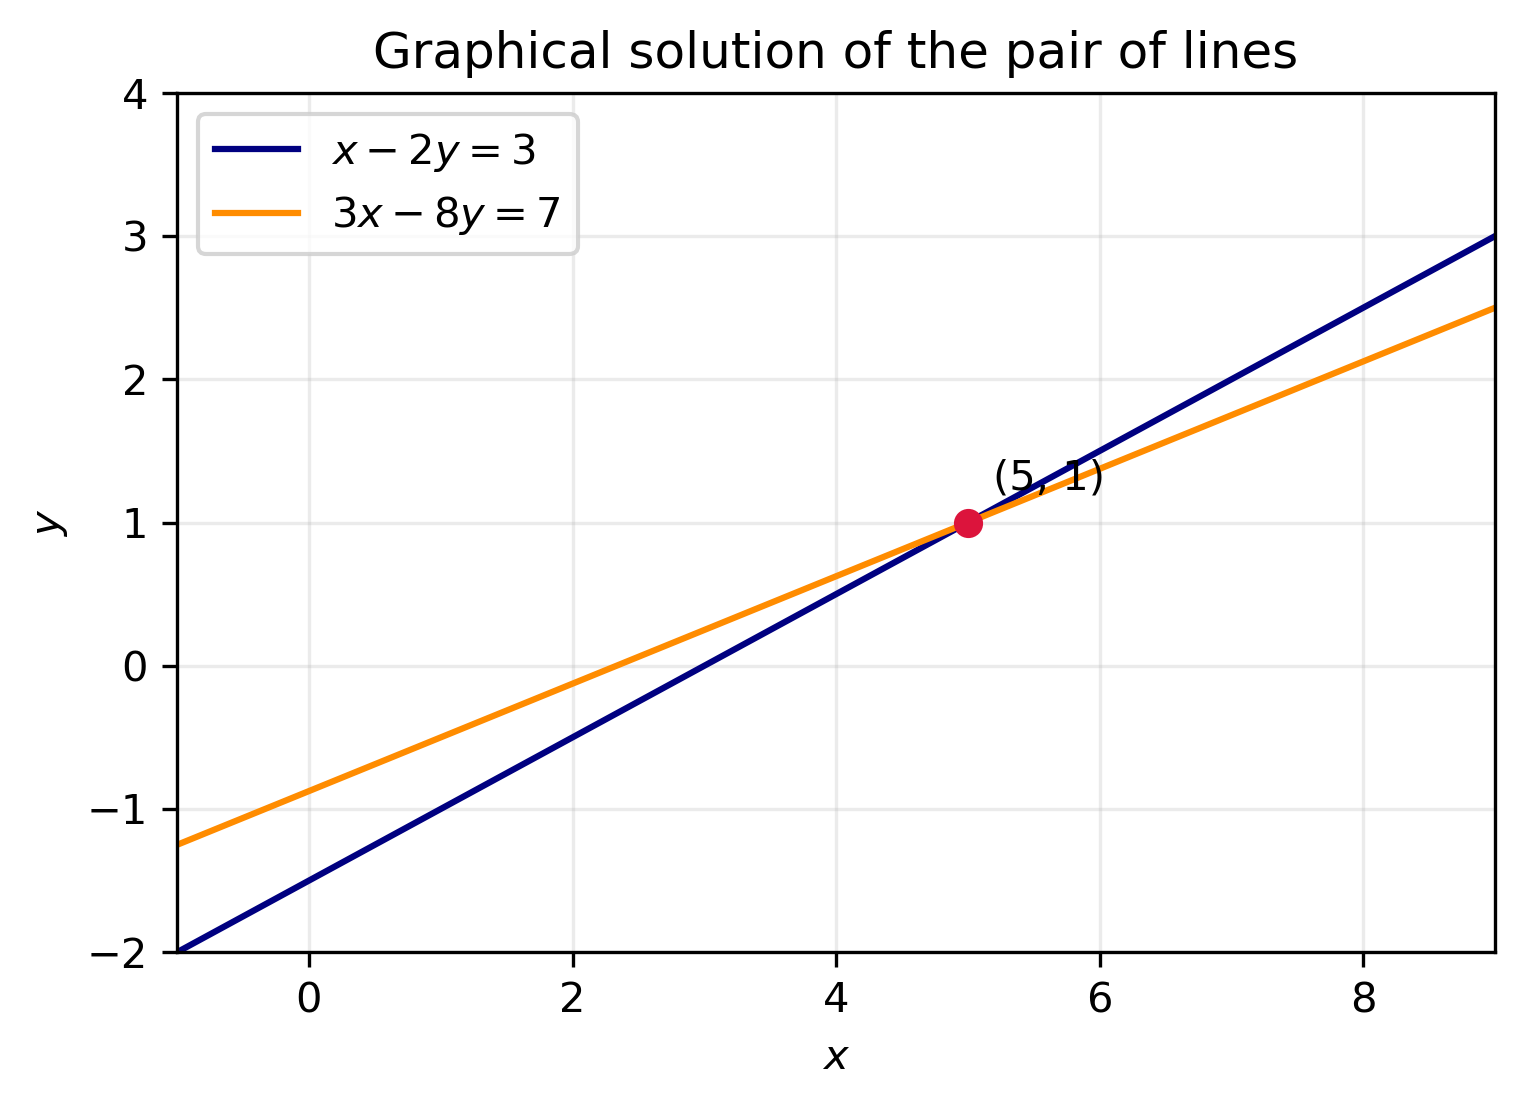
\includegraphics[width=0.52\linewidth]{figs/3.1.34.1.png}
    \caption{The lines intersect at $(5,1)$.}
\end{figure}

\item[3.1.35] A boy flies a kite with a $60$ m string at an elevation of $30^\circ$. Another boy on the roof of a $20$ m building sees the same kite at $45^\circ$. If the boys are on opposite sides of the kite, find the first boy's distance from the building and the kite's height from the ground. Use $\sqrt3=1.73$.

\vspace{0.6em}\par\noindent\textbf{Solution:}

The kite's height is $60\sin30^\circ=30$ m. From the rooftop boy's $45^\circ$ angle, the horizontal distance from the building to the kite is $30-20=10$ m. From the first boy to the kite the horizontal distance is $60\cos30^\circ=30\sqrt3$ m. Since the kite lies between the boys, the first boy is $30\sqrt3+10\approx61.9$ m from the building. The code plots the configuration.
\begin{lstlisting}[frame=single, basicstyle=\rmfamily, escapeinside={(*@}{@*)}]
(*@\makebox[\dimexpr\linewidth-2\fboxsep-2\fboxrule\relax][c]{codes/3.1.35.py}@*)
\end{lstlisting}
\begin{figure}[H]
    \centering
    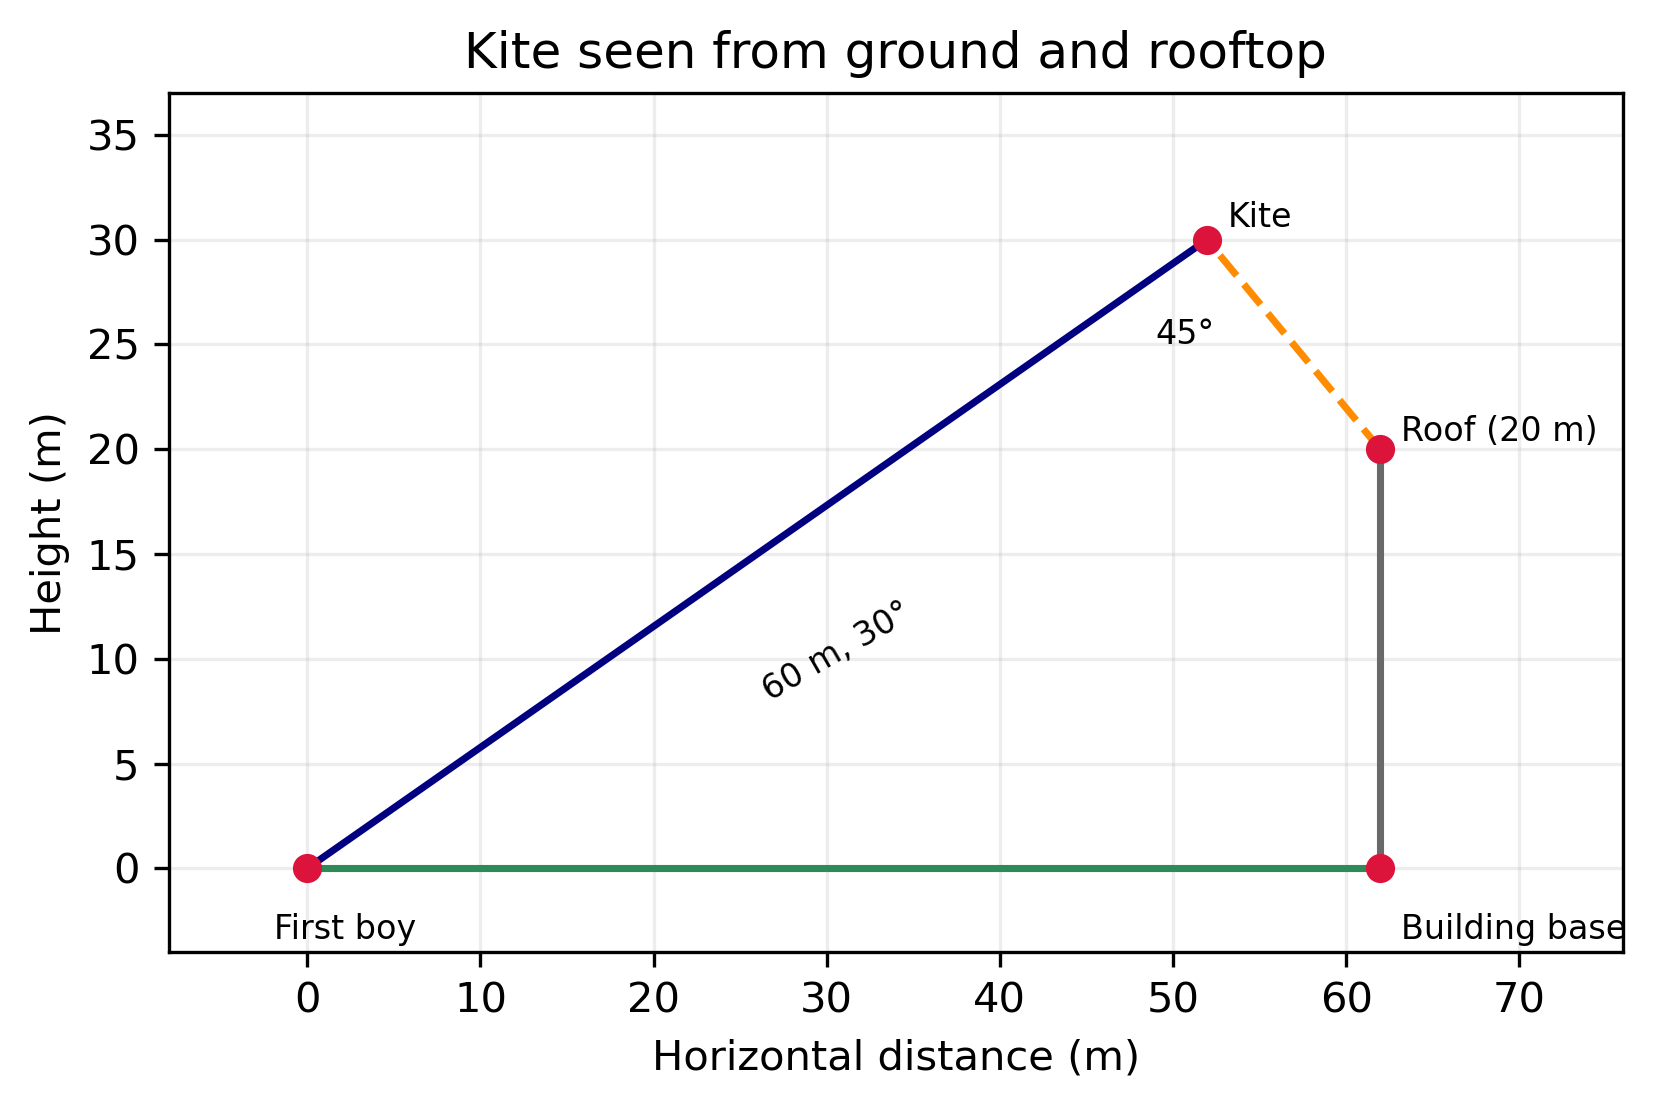
\includegraphics[width=0.58\linewidth]{figs/3.1.35.png}
    \caption{Kite position relative to the two observers.}
\end{figure}

\item[3.1.36] The arch is modelled by $p(x)=-x^2+2x+8$, where $x$ is distance along the stage. Find (i) its height, (ii)(a) its zeroes and the corresponding graph points, or (ii)(b) its span, and (iii) the point where it meets the $y$-axis.

\vspace{0.6em}\par\noindent\textbf{Solution:}

Writing $p(x)=-(x-1)^2+9$ shows the maximum height is $9$ ft. Factoring gives $p(x)=-(x-4)(x+2)$, so the zeroes are $-2$ and $4$, represented by $(-2,0)$ and $(4,0)$. The span between these intercepts is $6$ ft. At $x=0$, $p(0)=8$, so the $y$-intercept is $(0,8)$. The code plots the parabola and marks these points.
\begin{lstlisting}[frame=single, basicstyle=\rmfamily, escapeinside={(*@}{@*)}]
(*@\makebox[\dimexpr\linewidth-2\fboxsep-2\fboxrule\relax][c]{codes/3.1.36.py}@*)
\end{lstlisting}
\begin{figure}[H]
    \centering
    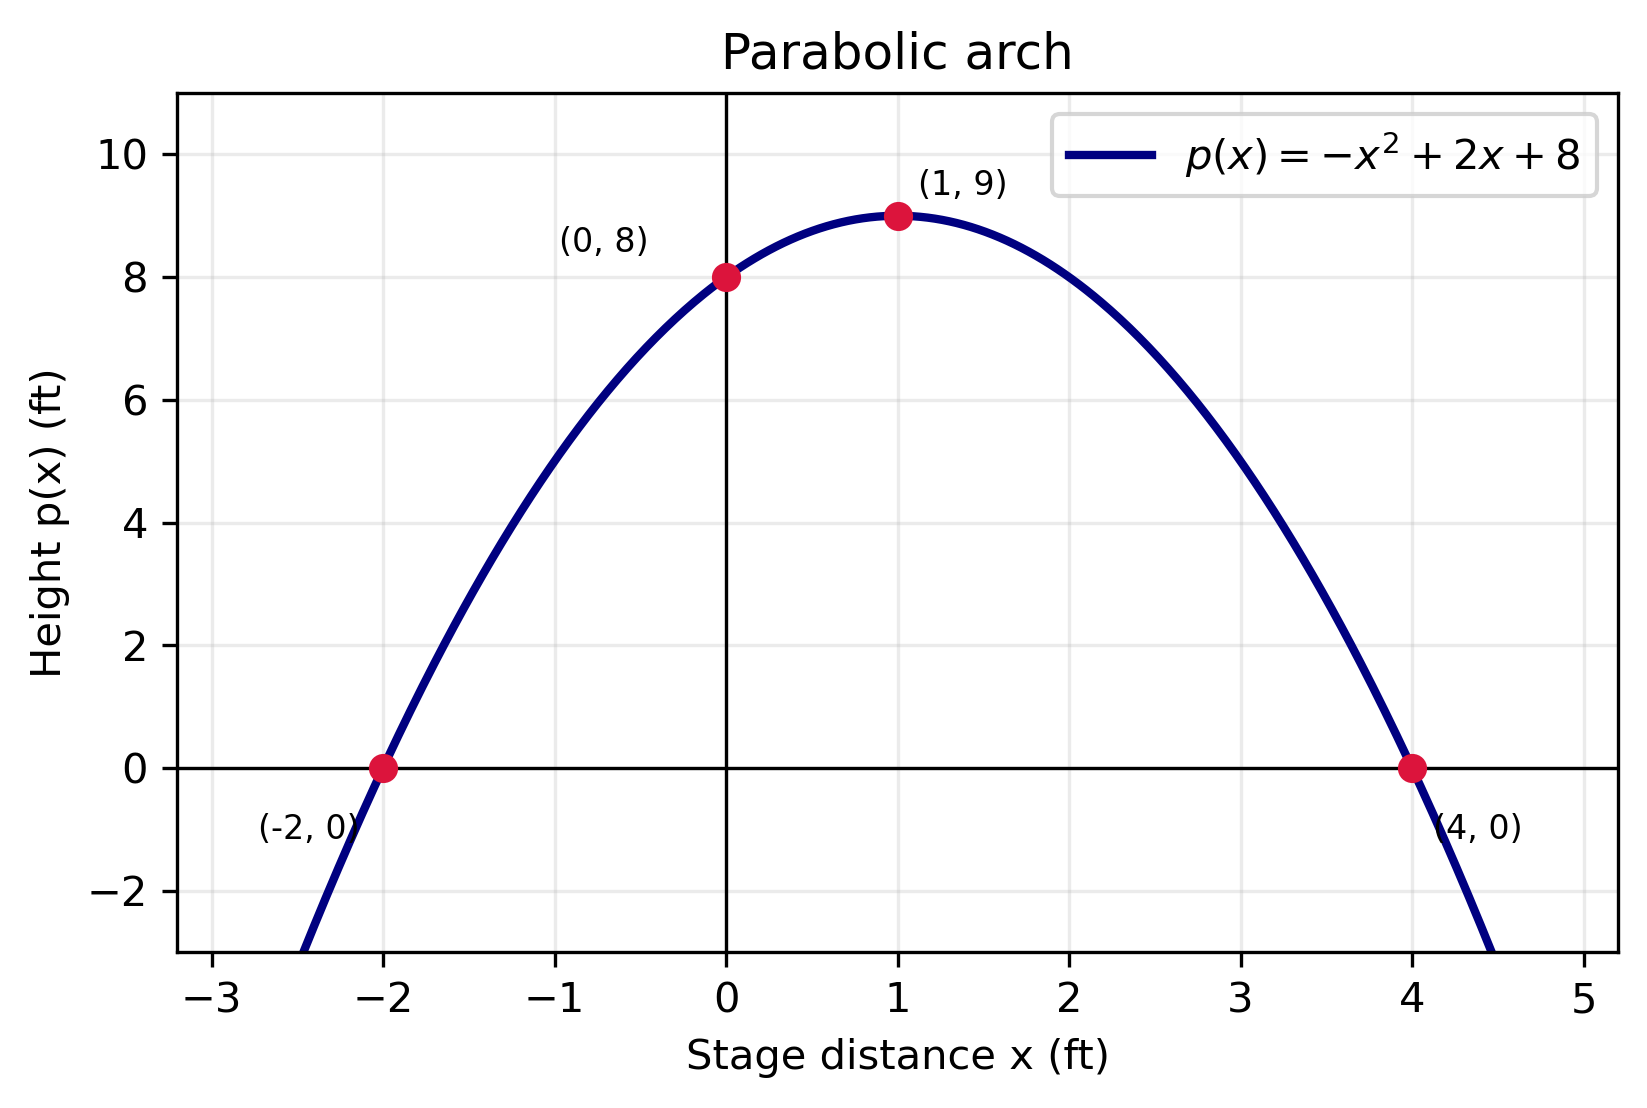
\includegraphics[width=0.56\linewidth]{figs/3.1.36.png}
    \caption{The arch polynomial and its intercepts and vertex.}
\end{figure}

\item[3.1.37] Three cards are dropped from two identical packs: a queen of hearts, a ten of spades, and an ace of clubs. One of the remaining cards is drawn at random. Find (i) the probability of a face card, (ii) the probability of a king or queen, (iii)(a) whether the probability of a queen would be higher if no cards were dropped, or (iii)(b) the probability of a jack and compare it with the probability when no cards were dropped.

\vspace{0.6em}\par\noindent\textbf{Solution:}

There are $104-3=101$ cards left. (i) Two packs have $24$ face cards; the dropped queen is one of them, leaving $23$, so $P(\text{face card})=23/101$. (ii) There are $16$ kings and queens altogether; one queen was dropped, so $P(\text{king or queen})=15/101$.

(iii)(a) After the drops, $P(\text{queen})=7/101$. With no drops it would be $8/104=2/13$. Since $7/101<2/13$, the probability would be higher with no cards dropped. (iii)(b) No jack was dropped, so with the drops $P(\text{jack})=8/101$; with no drops it is $8/104=2/26=1/13$. The probability of a jack is higher after the three non-jack cards are removed.

\item[3.1.38] A tabletop fountain has a spherical ball of diameter $21$ cm and a cylindrical pool with outer diameter $50$ cm and inner diameter $40$ cm. The solid base is $14$ cm high and water is $7$ cm deep. Find (i) the total height, (ii) the ball's volume, (iii)(a) the volume of water if one-third of the ball is submerged, or (iii)(b) the sum of the outer curved surface area of the cylinder and the ball's surface area.

\vspace{0.6em}\par\noindent\textbf{Solution:}

The radius of the ball is $10.5$ cm. (i) Its diameter sits above the $14$ cm base, giving a total height of $14+21=35$ cm. (ii) $V_{\text{ball}}=\frac43\pi(10.5)^3=1543.5\pi=4851$ cm$^3$ (using $\pi=22/7$).

(iii)(a) The water occupies a cylinder of inner radius $20$ cm and depth $7$ cm, less the submerged one-third of the ball:
\[
V_{\text{water}}=\pi(20)^2(7)-\frac13\left(\frac43\pi(10.5)^3\right)=2285.5\pi\approx7183\text{ cm}^3.
\]
(iii)(b) The outer cylinder is $14+7=21$ cm high, so its curved area is $2\pi(25)(21)=1050\pi$ cm$^2$. The ball's surface area is $4\pi(10.5)^2=441\pi$ cm$^2$. Their sum is $1491\pi\approx4686$ cm$^2$.
\end{list}

\end{document}
